% !TEX TS-program = xelatex

\documentclass[a4paper,twoside,11pt]{report} %openright
\newcommand{\documenttype}{Master Thesis}
\newcommand{\thesistitle}{Investigation of Deep Probibalistic Surrogate-models in Bayesian Optimization}
\newcommand{\thesissubtitle}{}

\newcommand{\thesisauthor}{Simon Saugmandsgaard Kruse} % Your name :) 
\newcommand{\studentnumber}{s164221}
\newcommand{\thedate}{June, 2022} % For example "June, 2019"

\newcommand{\department}{DTU Compute}
\newcommand{\departmentdescriber}{Section of Cognitive Systems}
\newcommand{\addressI}{Building 321}
\newcommand{\addressII}{2800 Kgs. Lyngby}
\newcommand{\departmentwebsite}{www.github.com/SimonKruse0/master-thesis}

%\usepackage{microtype}      % better looking text
%\usepackage[utf8]{inputenc}
\usepackage{fontspec}       % Package for custom fonts
\usepackage[]{geometry}     % Package for changing page margins (before fancyhdr) 
\usepackage{fancyhdr}       % Package to change header and footer
\usepackage{parskip}        % Package to tweak paragraph skipping (instead of indents a small skip is added after every paragraph)
\usepackage{titlesec}
\usepackage{tikz}           % Package for drawing
\usepackage{pgfplots}       % Package for creating graphs and charts
\usepackage{xcolor}         % Package for defining DTU colours to be used
\usepackage{amsmath}        % For aligning equations among other
\usepackage{siunitx}        % SI units
\usepackage{listings}       % Package for inserting code, (before cleveref)
\PassOptionsToPackage{hyphens}{url} % Ability to line break urls at hyphens
\usepackage{hyperref}       % Package for cross referencing (also loads url package)
\usepackage{cleveref}       % improved cross referencing
\usepackage{textcomp}       % \textdegree = °C and other useful symbols
\usepackage[english]{babel} % localisation 
\usepackage{caption}        % better captions
\usepackage{subcaption}     % for subfigures
\usepackage{csquotes}       % For biblatex with babel
\usepackage[backend=biber,style=numeric,sorting=none]{biblatex} % Package for bibliography (citing)
\bibliography{bibliography.bib}
\usepackage{tabularx}       % for ability to adjust column spacing in tabular better
\usepackage{booktabs}       % for better tables
\usepackage{float}          % floating figures in correct places
\usepackage{calc}           % Adds ability for latex to calculate (3pt+2pt) 
\usepackage{blindtext}
\usepackage{amssymb}
\usepackage{bm}
\usepackage{enumitem}
%\usepackage{floatrow}
\usepackage[percent]{overpic}
% Colours! 
\newcommand{\targetcolourmodel}{cmyk} % rgb for a digital version, cmyk for a printed version. Only use lowercase
\selectcolormodel{\targetcolourmodel}

% Define colours from https://www.designguide.dtu.dk/
\definecolor{dtured}    {rgb/cmyk}{0.6,0,0 / 0,0.91,0.72,0.23}
\definecolor{blue}      {rgb/cmyk}{0.1843,0.2431,0.9176 / 0.88,0.76,0,0}
\definecolor{brightgreen}{rgb/cmyk}{0.1216,0.8157,0.5098 / 0.69,0,0.66,0}
\definecolor{navyblue}  {rgb/cmyk}{0.0118,0.0588,0.3098 / 1,0.9,0,0.6}
\definecolor{yellow}    {rgb/cmyk}{0.9647,0.8157,0.3019 / 0.05,0.17,0.82,0}
\definecolor{orange}    {rgb/cmyk}{0.9882,0.4627,0.2039 / 0,0.65,0.86,0}
\definecolor{pink}      {rgb/cmyk}{0.9686,0.7333,0.6941 / 0,0.35,0.26,0}
\definecolor{grey}      {rgb/cmyk}{0.8549,0.8549,0.8549 / 0,0,0,0.2}
\definecolor{red}       {rgb/cmyk}{0.9098,0.2471,0.2824 / 0,0.86,0.65,0}
\definecolor{green}     {rgb/cmyk}{0,0.5333,0.2078 / 0.89,0.05,1,0.17}
\definecolor{purple}    {rgb/cmyk}{0.4745,0.1373,0.5569 / 0.67,0.96,0,0}

\newcommand{\dtulogocolour}{white} % Colour of the DTU logo: white, black or dtured
\newcommand{\frontpagetextcolour}{white} % front page text colour: white or black
\colorlet{frontbackcolor}{blue} % Set the background colour of the front- and back page. Choose the colour so it matches the main colour of front page picture

% DTU colours for diagrams
% You might want to make the front/back page background colour the first colour in the plot cycle list.
\pgfplotscreateplotcyclelist{DTU}{%
dtured,         fill=dtured,        \\%
blue,           fill=blue,          \\%
brightgreen,    fill=brightgreen    \\%
navyblue,       fill=navyblue       \\%
yellow,         fill=yellow         \\%
orange,         fill=orange         \\%
grey,           fill=grey           \\%
red,            fill=red            \\%
green,          fill=green          \\%
purple,         fill=purple         \\%
}


% Font
% There is no corporate serif font in the DTU design guide. The DTU design team has proposed to use Neo Sans for headings - and Arial for the body text.
% To change heading font to NeoSans Pro please upload both NeoSansPro-Regular.otf and NeoSansPro-Medium.otf to the root directory.
%\setmainfont{Arial}
\setmainfont{Times New Roman}
\renewcommand\thepart{Part \Roman{part}}
\IfFontExistsTF{NeoSansPro-Medium.otf}
{ %If True set headings to NeoSans Pro
\newfontface\NeoSansProReg{NeoSansPro-Regular.otf}
\newfontface\NeoSansProMed{NeoSansPro-Medium.otf}
\titleformat{\part}[display]{\NeoSansProMed \huge \centering}{\NeoSansProMed \Huge \thepart}{1em}{\thispagestyle{empty}}{}
\titleformat{\chapter}{\NeoSansProMed\huge}{\thechapter}{1em}{\raggedright}
\titleformat{\section}{\NeoSansProMed\Large}{\thesection}{1em}{\raggedright}
\titleformat{\subsection}{\NeoSansProMed\large}{\thesubsection}{1em}{\raggedright}
\titleformat{\subsubsection}{\NeoSansProMed\normalsize}{\thesubsubsection}{1em}{\raggedright}
\newcommand\TitleFont[1]{{\NeoSansProMed #1}}
\newcommand\titlefont[1]{{\NeoSansProReg #1}}
}
{ % If false
\titleformat{\part}[display]{\bfseries\huge \centering}{\bfseries\Huge \thepart}{1em}{\thispagestyle{empty}}{}
\titleformat{\chapter}{\bfseries\huge}{\thechapter}{1em}{\raggedright}
\titleformat{\section}{\bfseries\Large}{\thesection}{1em}{\raggedright}
\titleformat{\subsection}{\bfseries\large}{\thesubsection}{1em}{\raggedright}
\titleformat{\subsubsection}{\bfseries\normalsize}{\thesubsubsection}{1em}{\raggedright}
\newcommand\TitleFont[1]{{\bfseries #1}}
\newcommand\titlefont[1]{{#1}}
}
\urlstyle{sf}
%\def\UrlFont{\NeoSansProReg}


% If you wish to use the pdflatex compiler, sans-serif Helvetica can be used as a replacement for Arial. In this way you will be able to use the microtype package. Remember to add \usepackage[utf8]{inputenc} and disable the fontspec package. 
%\newcommand\TitleFont[1]{{\bfseries #1}}
%\newcommand\titlefont[1]{{#1}}
%\fontfamily{qhv}\selectfont
%\renewcommand{\familydefault}{\sfdefault}


% Table of contents (TOC) and numbering of headings
\setcounter{tocdepth}{1}    % Depth of table of content: sub sections will not be included in table of contents
\setcounter{secnumdepth}{2} % Depth of section numbering: sub sub sections are not numbered

\makeatletter % Reset chapter numbering for each part
\@addtoreset{chapter}{part}
\makeatother  

% Spacing of titles and captions
\titlespacing\chapter{0pt}{0pt plus 4pt minus 2pt}{4pt plus 2pt minus 2pt}
\titlespacing\section{0pt}{12pt plus 3pt minus 3pt}{2pt plus 1pt minus 1pt}
\titlespacing\subsection{0pt}{8pt plus 2pt minus 2pt}{0pt plus 1pt minus 1pt}
\titlespacing\subsubsection{0pt}{4pt plus 1pt minus 1pt}{-2pt plus 1pt minus 1pt}
\captionsetup{belowskip=\parskip,aboveskip=4pt plus 1pt minus 1pt}

% Setup header and footer
\fancypagestyle{main}{% All normal pages
    \fancyhead{}
    \fancyfoot{}
    \renewcommand{\headrulewidth}{0pt}
    \fancyfoot[LE,RO]{\footnotesize \thepage}
    \fancyfoot[RE,LO]{\footnotesize \thesistitle} % - \rightmark
    \fancyhfoffset[E,O]{0pt}
}
\fancypagestyle{plain}{% Chapter pages
    \fancyhead{}
    \fancyfoot{}
    \renewcommand{\headrulewidth}{0pt}
    \fancyfoot[LE,RO]{\footnotesize \thepage}
    \fancyfoot[RE,LO]{\footnotesize \thesistitle} % - \leftmark
    \fancyhfoffset[E,O]{0pt}
}


% Setup for diagrams and graphs (tikz pictures) 
\usetikzlibrary{spy}    % For magnifying anything within a tikzpicture, see the line graph
\usepgfplotslibrary{statistics} % Package for the boxplot
\pgfplotsset{ % Setup for diagrams
compat=newest,
major x grid style={line width=0.5pt,draw=grey},
major y grid style={line width=0.5pt,draw=grey},
legend style={at={(0.5,-0.1)}, anchor=north,fill=none,draw=none,legend columns=-1,/tikz/every even column/.append style={column sep=10pt}},
axis line style={draw=none},
tick style={draw=none},
every axis/.append style={ultra thick},
tick label style={/pgf/number format/assume math mode}, % To apply main font to tick labels (numbers on the axis)
}
\tikzset{every mark/.append style={scale=1.5}}


% Hypersetup
\hypersetup{
    pdfauthor={\thesisauthor},
    pdftitle={\thesistitle},
    pdfsubject={\thesissubtitle},
    pdfdisplaydoctitle,
    bookmarksnumbered=true,
    bookmarksopen,
    breaklinks,
    linktoc=all,
    plainpages=false,
    unicode=true,
    colorlinks=false,
    hidelinks,                        % Do not show boxes or coloured links.
}


% Listings setup
\lstset{
    basicstyle=\footnotesize\ttfamily,% the size of the fonts that are used for the code
    commentstyle=\color{green},       % comment style
    keywordstyle=\bfseries\ttfamily\color{blue}, % keyword style
    numberstyle=\sffamily\tiny\color{grey}, % the style that is used for the line-numbers
    stringstyle=\color{purple},       % string literal style
    rulecolor=\color{grey},           % if not set, the frame-color may be changed on line-breaks within not-black text (e.g. comments (green here))
    breakatwhitespace=false,          % sets if automatic breaks should only happen at whitespace
    breaklines=true,                  % sets automatic line breaking
    captionpos=b,                     % sets the caption-position to bottom
    deletekeywords={},                % if you want to delete keywords from the given language
    escapeinside={\%*}{*)},           % if you want to add LaTeX within your code
    frame=single,                     % adds a frame around the code
    xleftmargin=4pt, 
    morekeywords={*,...},             % if you want to add more keywords to the set
    numbers=left,                     % where to put the line-numbers; possible values are (none, left, right)
    numbersep=10pt,                   % how far the line-numbers are from the code
    showspaces=false,                 % show spaces everywhere adding particular underscores; it overrides 'showstringspaces'
    showstringspaces=false,           % underline spaces within strings only
    showtabs=false,                   % show tabs within strings adding particular underscores
    stepnumber=1,                     % the step between two line-numbers. If it's 1, each line will be numbered
    tabsize=2,                        % sets default tabsize to 2 spaces
    title=\lstname,                   % show the filename of files included with \lstinputlisting; also try caption instead of title
}

% Signature field
\newlength{\myl}
\newcommand{\namesigdatehrule}[1]{\par\tikz \draw [black, densely dotted, very thick] (0.04,0) -- (#1,0);\par}
\newcommand{\namesigdate}[2][]{%
\settowidth{\myl}{#2}
\setlength{\myl}{\myl+10pt}
\begin{minipage}{\myl}%
\begin{center}
    #2  % Insert name from the command eg. \namesigdate{\authorname}
    \vspace{1.5cm} % Spacing between name and signature line 
    \namesigdatehrule{\myl}\smallskip % Signature line and a small skip
    \small \textit{Signature} % Text under the signature line "Signature"
    \vspace{1.0cm} % Spacing between "Signature" and the date line
    \namesigdatehrule{\myl}\smallskip % Date line and a small skip
    \small \textit{Date} % Text under date line "Date" 
\end{center}
\end{minipage}
}

% For the back page: cleartoleftpage
\newcommand*\cleartoleftpage{%
  \clearpage
  \ifodd\value{page}\hbox{}\newpage\fi
}

\usepackage{Setup/MoreSettings}

\begin{document}

\pagenumbering{roman}
\title{\thesistitle} 
\author{\thesisauthor} 
\date{\thedate} 

\begin{titlepage}

\newgeometry{left=11mm,right=11mm,top=50mm,bottom=0pt}
\pagecolor{frontbackcolor}
\color{\frontpagetextcolour}

\begin{flushleft}
{ % Thesis title (to change see Setup/Settings.tex) 
\Huge
\begin{tabular}{p{\linewidth}}
%\TitleFont{\thesistitle}   \\ 
\TitleFont{Investigation of Deep Probabilistic Surrogate-}\\
\TitleFont{models in Bayesian Optimization} \bigskip \\ 
%\titlefont{\thesissubtitle} \bigskip \\ 
{\huge Simon Saugmandsgaard Kruse}\\
{\LARGE \documenttype}\\
\end{tabular}
}
\end{flushleft} 

% DTU department (to change see Setup/Settings.tex) 
\begin{tikzpicture}[remember picture,overlay]
\node[anchor=north east, 
      xshift=-10mm, 
      yshift=-12mm] 
      at (current page.north east) 
      {
        \color{\frontpagetextcolour}
        \begin{tabular}{r} 
        \textbf{\department} \\ 
        \departmentdescriber
        \end{tabular}
      }; 
\end{tikzpicture}

% DTU logo
\begin{tikzpicture}[remember picture,overlay]
\node[anchor=north west, 
      xshift=8.9mm, 
      yshift=-8.3mm] 
     at (current page.north west) 
     {\includegraphics[width=14.75mm,keepaspectratio]{Pictures/Logos/\dtulogocolour_\targetcolourmodel.pdf}}; 
\end{tikzpicture}

% Cover photo
% \begin{tikzpicture}[remember picture,overlay]
% \node[anchor=south, % anchor is bottom of picture
%       xshift=0pt, 
%       yshift=-2.9mm] % shifting picture to actually be at the bottom of the page
%      at (current page.south) % placement at bottom of the page
%      {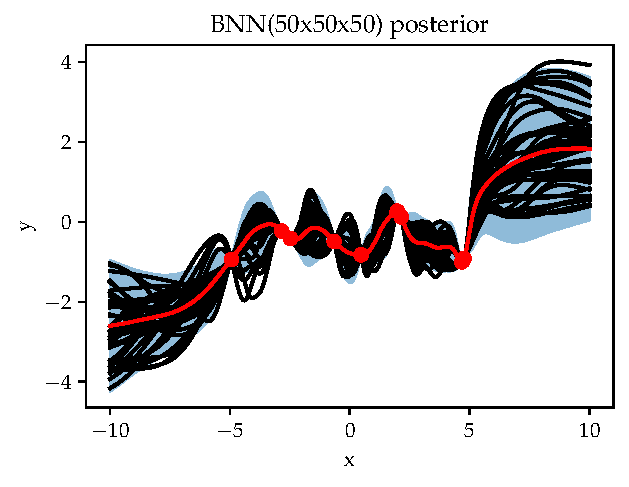
\includegraphics[height=18.9cm,keepaspectratio]{Pictures/BNN_posterior.pdf}};
% \end{tikzpicture}

\tikzset{every picture/.style={line width=0.75pt}} %set default line width to 0.75pt        

\begin{tikzpicture}[remember picture,overlay]
      \node[anchor=south, % anchor is bottom of picture
            xshift=-15mm, 
            yshift=30mm]
            at (current page.south){
            %\path (0,310); %set diagram left start at 0, and has height of 310
            \resizebox{1.34\textwidth}{!}{%
            \begin{tikzpicture}[x=0.55pt,y=1.25pt,yscale=-1,xscale=1]
              %Curve Lines [id:da9880396283111128] 
              \draw    (-3,149) .. controls (37,119) and (631,152) .. (671,122) ;
              %Shape: Free Drawing [id:dp07450350989511567] 
              \draw  [color={rgb, 255:red, 0; green, 0; blue, 0 }  ,draw opacity=1 ][line width=3] [line join = round][line cap = round] (1,217) .. controls (9.22,217) and (16.92,223.69) .. (25,226) .. controls (41.54,230.73) and (74.95,221.05) .. (87,209) .. controls (105.26,190.74) and (119.38,166.92) .. (134,145) .. controls (139.73,136.41) and (145.18,124.73) .. (154,119) .. controls (162.38,113.56) and (171.87,110.06) .. (181,106) .. controls (194.08,100.19) and (206.2,94.54) .. (221,94) .. controls (252.1,92.87) and (283.1,92.65) .. (313,102) .. controls (325.49,105.9) and (359.46,131.87) .. (369,138) .. controls (378.91,144.37) and (389.67,149.33) .. (400,155) .. controls (427.23,169.93) and (448.29,187.48) .. (479,198) .. controls (503.38,206.35) and (531.3,202.09) .. (556,199) .. controls (595.29,194.09) and (632.75,185.23) .. (672,184) ;
              %Shape: Free Drawing [id:dp6323192319779791] 
              \draw  [line width=3] [line join = round][line cap = round] (-5.92,100) .. controls (-2.51,100) and (6.86,94.78) .. (9.33,96) .. controls (17.1,99.82) and (23.07,109.05) .. (32.7,108) .. controls (40.32,107.17) and (44.09,97.82) .. (48.97,92) .. controls (49.4,91.49) and (48.97,89.33) .. (48.97,90) .. controls (48.97,102.37) and (56.01,118.15) .. (60.15,129) .. controls (60.26,129.31) and (76.41,110) .. (76.41,110) .. controls (76.41,110) and (80.82,124.16) .. (81.49,127) .. controls (84.55,140.04) and (89.44,152.65) .. (94.7,165) .. controls (95.54,166.97) and (97.67,161.84) .. (98.77,160) .. controls (101.4,155.57) and (111.47,139.87) .. (116.05,141) .. controls (119.15,141.76) and (119.5,146.29) .. (121.13,149) .. controls (129.92,163.6) and (136.07,175.33) .. (149.59,185) .. controls (158.99,191.73) and (162.41,187.67) .. (168.9,182) .. controls (171.5,179.72) and (175.69,174.47) .. (178.04,177) .. controls (190.74,190.63) and (200.54,205.13) .. (218.7,212) .. controls (224,214.01) and (231.73,204.77) .. (233.94,203) .. controls (246.38,193.06) and (257.18,181.7) .. (260.37,166) .. controls (260.8,163.91) and (262.66,169.78) .. (264.44,171) .. controls (269.67,174.61) and (274.92,178.31) .. (280.7,181) .. controls (292.33,186.42) and (312.48,194.15) .. (326.43,189) .. controls (333.1,186.54) and (332.01,176.06) .. (335.58,170) .. controls (337.02,167.55) and (339.98,166.28) .. (341.68,164) .. controls (343.92,160.99) and (346.76,154) .. (346.76,154) .. controls (346.76,154) and (350.46,159.64) .. (352.86,162) .. controls (358.69,167.74) and (366.25,173.74) .. (375.22,173) .. controls (391.02,171.7) and (401.03,149.88) .. (407.74,139) .. controls (411.3,133.23) and (415.86,128.04) .. (418.92,122) .. controls (420.99,117.94) and (421.34,113.23) .. (422.99,109) .. controls (425.17,103.42) and (424.76,112.05) .. (432.14,117) .. controls (437.52,120.61) and (443.28,123.83) .. (449.42,126) .. controls (457.24,128.77) and (473.31,123.11) .. (479.91,120) .. controls (490.71,114.92) and (506.25,108.08) .. (514.46,100) .. controls (519.38,95.16) and (524.15,90.18) .. (528.69,85) .. controls (530.02,83.49) and (532.26,77.7) .. (535.81,77) .. controls (543.28,75.53) and (543.2,83.93) .. (548,90) .. controls (553.94,97.51) and (566.06,101.59) .. (575.44,98) .. controls (588.4,93.04) and (603.28,84.05) .. (615.08,77) .. controls (619.26,74.51) and (623.3,71.79) .. (627.28,69) .. controls (628.06,68.45) and (628.35,67) .. (629.31,67) .. controls (630.84,67) and (638.51,73.56) .. (639.48,74) .. controls (642.42,75.35) and (653.36,77.33) .. (656.75,80) .. controls (659.19,81.92) and (659.73,87) .. (662.85,87) .. controls (664.25,87) and (665.56,86.33) .. (666.92,86) ;
            \end{tikzpicture}
            }%  
            };
      \end{tikzpicture}


\end{titlepage}

\pagecolor{white}
\newgeometry{top=2.81cm, bottom=2.75cm, outer=2.5cm, inner=3.5cm}
\pagestyle{empty}
\cleardoublepage 
\thispagestyle{empty}
\setcounter{page}{1}
\vspace*{\fill}

\textbf{\thesistitle} \newline
\thesissubtitle

\smallskip

\documenttype \newline
\thedate

\smallskip

By \newline
\thesisauthor

\bigskip

\begin{tabularx}{\textwidth}{@{}lX@{}}
    Copyright: & Reproduction of this publication in whole or in part must include the customary bibliographic citation, including author attribution, report title, etc. \\
    Cover photo: & Vibeke Hempler, 2012 \\
    Published by: & DTU, \departmentdescriber, \addressI, \addressII ~Denmark  \\
     & \url{\departmentwebsite} \\
    ISSN: & [0000-0000] (electronic version) \\
    ISBN: & [000-00-0000-000-0] (electronic version) \\
    & \\
    ISSN: & [0000-0000] (printed version) \\
    ISBN: & [000-00-0000-000-0] (printed version)
\end{tabularx}



\clearpage 
\pagestyle{main}
\section*{Approval}
\addcontentsline{toc}{section}{Preface}
This master thesis was prepared at the Section of Cognitive Systems at the Technical University of Denmark in
fulfillment of the requirements of the degree Master of Science in Engineering, MSc Eng, in Mathematical Modeling and Computation.

%The work was carried out in the spring of 2022 and project covers a work load of 30 ects point. 
\vfill

\begin{center}
\namesigdate{\thesisauthor~-~\studentnumber}
\end{center}

\vfill


\clearpage 
\section*{Abstract}
\addcontentsline{toc}{section}{Abstract}
% Abstract
%  1. Motivation. Why do we care?
Bayesian optimization is the leading way in sample efficient optimization. Tuning
hyper parameters in machine learning and deep learning. 

%  2. Problem formulation. What problem will we solve?
%     2.b. Current state. What have others done, and why is that not enough?
However, from a decision theretically standpoint, assuming the probalistic surrogate model to be correct 
is crucial for the correct decision. We will investigate if other surrogate models 
could be better than a GP. 

%  3. Approach. What is our big idea? How did we solve it?
%     3.a. Analysis and experiments. What research did we do?
Mixture regression, and SPN, modeling the trying out BNN.

%  4. Results. What is the answer?
%  5. Conclusions. What are the implications?







\clearpage 
hej
\section*{Acknowledgements}
\addcontentsline{toc}{section}{Acknowledgements}
\textbf{\thesisauthor}, MSc Civil Engineering, DTU \newline
Creator of this thesis template.

\textbf{S. Tejs K.} \newline

\textbf{[Name]}, [Title], [affiliation] \newline
[text]


\cleardoublepage 
\tableofcontents
\cleardoublepage 

%%%%%%%%%%%%%%%%%%%%%%%%%%%%%%%%%%%%%%%%%%%%%%%%%%%%%%%
\pagenumbering{arabic}

\chapter{Introduction}
% Introduction section
%  1. Introduction.
%  2. Background and setting. 
%  3. Identification of problem
%  4. Purpose Statement. 
%  5. Objectives or research questions
%  6. Assumptions. Limitations. Definition of terms
%  7. Significance of the study.

% Introduction section (from unsw.edu.au)
% Move A: establish your territory (say what the topic is about)
%   1.  state the general topic and give some background
%   2.  provide a review of the literature related to the topic
%   3.  define the terms and scope of the topic
Optimization plays an important part in our everyday life, science development, product design, and
much more. Examples of optimization could be choosing the optimal way to commute from A to B,
deciding what songs should land on your playlist, or constructing the strongest possible bridge using
limited material. In general, optimization is the art of choosing the best decision among a set of possible
decisions. Often we try to quantify how good a decision is: A bus takes 20 min, a car takes 15 min to go from A to B, How would
you rate the song? This bridge construction costs 10 million kroner. If it is possible to come up with a
quantification of how good a decision is in terms of a real number, then we can define the optimization problem as
\textit{mathematical} optimization problem: 
$$\min_{x\in \mathcal{X}} f(x)$$ where the functional $f: \mathcal{X} \rightarrow \mathbb{R}$ is
called the objective function and $\mathcal{X}$ is the set of possible decisions (or decisions you
consider). Note that the optimization problem is formulated as a minimization problem. If one identifies
the optimal decision as a maximum of $f$ (instead of the minima), then finding the minima in the
negating the objective function $-f(x)$ is equivalent. Throughout this thesis, we refer to
optimization as minimizing the objective function. The optimization problem is now in the domain of 
numbers and here many algorithms have been developed to find the minimum of the function
$f(\cdot)$.

Evaluation of the objective function can be cheap (e.g. if it just requires summing/multiplying
numbers) or highly expensive (e.g. if it involves human rating, large simulation, or physical
experiments). In the latter case, we want to avoid evaluating the objective function as much as
possible - we want to use \textit{sample efficient} optimization. The overall topic of this
thesis, \textit{Bayesian optimization}, is one of the preferred frameworks for sample efficient optimization. 

Bayesian optimization is a probabilistic surrogate-based optimization methodology: Assuming some samples from a
highly expensive objective, then a cheap (surrogate) function is used to fit the samples. The next sample
is found by minimizing the surrogate and the process is repeated. Bayesian optimization seeks to
enhance this procedure with probability theory, where the surrogate function becomes a probabilistic (Bayesian)
regression model. The most common choice is a Gaussian Process, as it encapsulates the uncertainty very well,
but also because its inference procedure (computing answers to probability queries like $p(y|x)$) is exact.

% Move B: establish a niche (show why there needs to be further research on your topic)
%   4.  outline the current situation
%   5.  evaluate the current situation (advantages/ disadvantages) and identify the gap

Even though GP has proven good for many cases, there will be problems where its assumptions do not
hold. E.g the commonly seen GP with an isotropic kernel (covariance between two points is invariant to
translation in input), yields a strong assumption about the continuity of the objective function and that
the objective function behaves similarly throughout the domain $\mathcal{X}$. In Figure
\ref{fig:GP_vs_BNN} we see an example of how the GP's uncertainty quantification is going wild due
to a discontinuity in the underlying objective function (a small varying step-function). In some areas is it very common to have
these discontinuities, for instance, in material discovery where it is well known that materials often
change very suddenly \cite{Nature_BO_paper}. To accommodate these challenges the literature introduces more
flexible kernel functions for the GP, however, this introduces additional hyperparameters and since
we often only deal with a small amount of data, tuning and computation can be significantly challenging \cite{Nature_BO_paper}.

\begin{figure}[H]%
    \centering
    {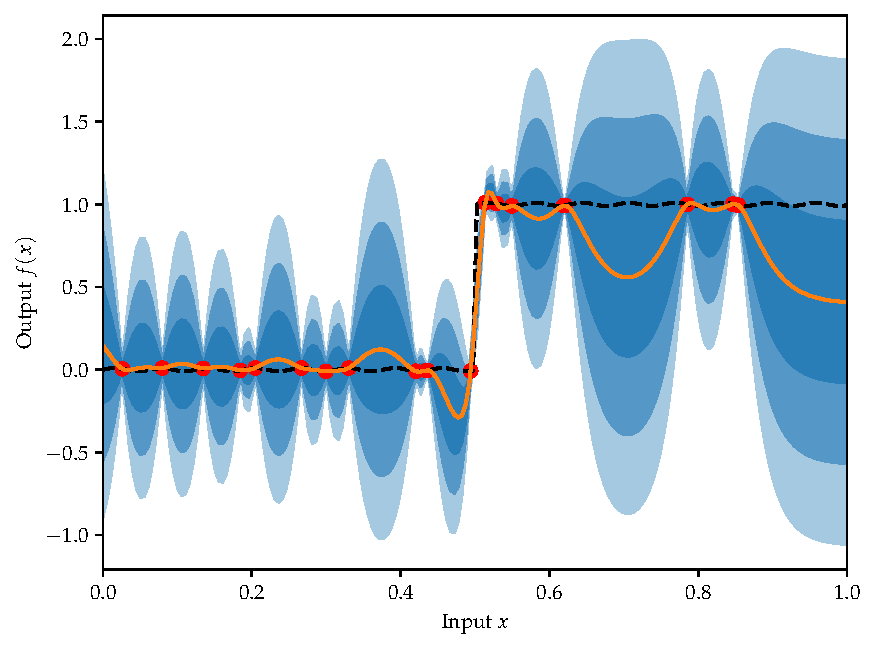
\includegraphics[width=0.46\textwidth]{Pictures/GP_vs_BNN1.pdf} }%
    \qquad
   {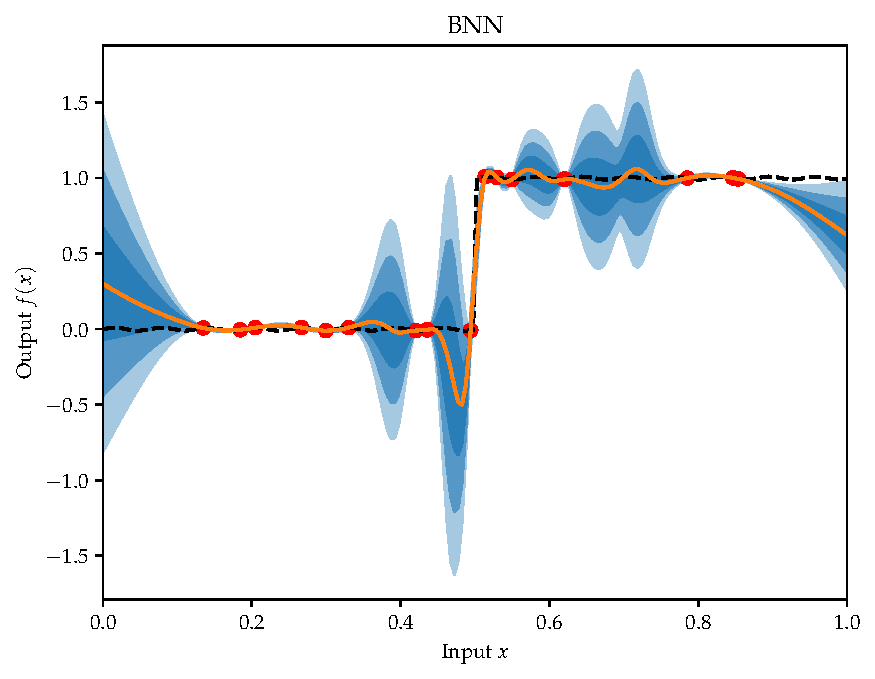
\includegraphics[width=0.46\textwidth]{Pictures/GP_vs_BNN2.pdf} }%
    \caption{Left: GP fitted to 20 data points. Right: A Bayesian neural network fitted to the same points.
    The objective function is the dashed black line. This examplifies how a discontinuerity makes the 
    standard implemented GP (optimized with emperical bayes) overreact to all other areas in the domain $[0,1]$,
    while the Bayesian NN only express uncertainty where the discontinuerity happen $x = 0.5$}%
    \label{fig:GP_vs_BNN}
\end{figure}


% Move C: introduce the current research (make hypotheses; state the research questions)
%   6.  identify the importance of the proposed research
%   7.  state the research problem/ questions
%   8.  state the research aims and/or research objectives
%   9.  state the hypotheses
%   10. outline the order of information in the thesis
%   11. outline the methodology

GPs are very attractive models since they allow for exact inference, a closed-form expected improvement (more on this later)
 and in general good uncertainty quantification.
However, as we saw in the figure \ref{fig:GP_vs_BNN} maybe we can do better! 
If it is possible to sample a few times less from the objective function, it can potentially
save hours of work, lots of money, or energy (Depending on what is demanded to evaluate the objective
function). It is therefore relevant to investigate if other models will perform better. As
mentioned, the assumptions of GP can be too strong. In this thesis, we aim to create models with less strong
assumptions, which can perform better on certain types of (complex) problems, and just as well as the GP on most types of  
problems. 

\section{Contribution}
This thesis investigates surrogate models alternative to GP, more concretely Bayesian NN
and mixture regression. The proposed hypotheses are,
\begin{enumerate}
    \item Neural Networks perform better applied to complex BO problems than GPs.
    \item Mixture regression models like SPN can be employed as an effective surrogate model
    performing better than GPs and Neural Networks in some complex cases. 
\end{enumerate}

Note what is meant by performance is \textit{sample efficiency}, i.e. how few evaluations of the objective function
are necessary to find the minima. So even though the surrogate modeling and optimization can be really slow, 
it is assumed that the objective function is very expensive, so a slow surrogate model would not matter.

% 1) Firstly, we want to examine what types of problems a GP surrogate is not a good choice and
% where Bayesian neural nets (BNN) surrogates can have an advantage (inspiration found in this 2020
% thesis \cite{PhDthesis})
    
% 2) Looking at sum product networks (SPN) as novel surrogate models. A SPN is - similarly to a BNN
% - a deep probabilistic model and still expressive but with tractable inference, which potentially
% could lead to advantages over BNNs. 

\section{Related work}
Here we give a short overview of research in different surrogates for Bayesian optimization
and the very related field active learning. The different surrogate models, which are in the 
research we found, 
\begin{itemize}
    \item Gaussian Process
    \item Bayesian neural network
    \item Random forest
    \item Kernel estimator
    \item Bayesian multivariate adaptive regression splines (BMARS)
    \item Bayesian additive regression trees (BART)
\end{itemize}

Often the main focus has been on lowering the computational complexity of inference while
showing performance is (or almost is) as well as GPs. Inference time of the GP scales cubic with the
number of data points and only linear for Bayesian Neural Network. Lowering the inference time is also the
main focus of the Ph.D. thesis "Sample-efficient Optimization Using Neural Networks" from 2020
\cite{PhDthesis}, but chapter 3 showcases empirically that using Bayesian neural networks as
surrogate models performed better, or at least comparable to GPs on a wide number of
problems. The performance difference was more clear for high-dimensional problems. 
<mention BOHAMIANN and DNGO>

The 2021 nature paper "Bayesian optimization with adaptive surrogate models for automated experimental design"
\cite{Nature_BO_paper}, focus on the sample efficiency of the BO applied to autonomous materials discovery, 
which yields a relatively high-dimensional design space and non-smooth patterns of objective functions.  
The paper shows that using Bayesian multivariate adaptive regression splines
and Bayesian additive regression trees as alternative surrogate models outperform GP significantly, 
for complex BO problems. 

Active learning is closely related to Bayesian Optimization, but here the focus is on learning the underlying function
using as few samples as possible instead of just finding its minima. 
In active learning, a Gaussian process is also very common, but the paper "Active Learning with Statistical Models" \cite{ALStatisticalModels}
investigates using Gaussian mixtures and kernel estimitor in active learning, i.e. as a surrogate model for selecting
the next samples. These are regression models not seen much in the literature, which
is modeling the joint distribution of x and y, and using the conditional distribution $p(y|x)$
as the regression model. The results were ... ??

\section{Structure of the thesis}
The structure of the thesis is
\begin{itemize}
    \item The first chapter introduces the concept of optimization in general, Bayesian optimization 
    and how surrogates/Bayesian regression models are relevant.
    \item The second chapter introduces GP and Bayesian Neural Networks
    \item The third chapter introduces the mixture regression and the novel new SPN regression.
    \item The fourth chapter results
    \item Finally a discussion and conclusion.
\end{itemize}
% Introduction to Optimization, and Bayesian optimization. 
% Presentation of different surrogate models. 
% Experiments using the different surrogates. 



% \section{No free lunch and surrogate reseach}

% <No free lunch theorem for optimization>, establish some questions on why there is no best method.
% And a burning research problem is if it is possible to use a different surrogate model than the GP. 
% And whether or not they in general performs better? What assumptions underlie the problem. 
% The assumption for GP regression is that the objective function follows a Gaussian process, whereas
% we assume it follows a random forest or neural network. These are assumptions that yields, consideration:
% Is this a good assumption? Bayesian NNs are very expressive. 

%   10. outline the order of information in the thesis
%   11. outline the methodology


% \section{Old intro}
% %<What is optimization>
% Optimization plays an important part in our everyday life, science development, and product design.
% What different transportation should you choose to get fast from A to B, what songs should
% land on your playlist, and what is the optimal bridge construction. Mathematical optimization problems 
% are all problems in the form, 
% $$\min_{x\in \mathcal{X}} f(x)$$ where $f: \mathcal{X} \rightarrow \mathcal{R}$ is a functional. I.e
% if it is possible to set up an objective function. e.g. what is the cost of the bridge given a
% specific design, or how pleasant you think some music, and some constraints such that you keep in
% the domain of interest. Evaluation of the objective function can be cheap e.g. if it just requires
% summing and multiplying numbers or highly expensive if it involves human rating or large simulation
% and physical experiments. Bayesian optimization is a preferred <ref> framework for optimization of
% the expensive objective functions. And is also referred to as \textit{sample efficient}
% optimization. 
% %<Why Bayesian optimization?>

% Bayesian optimization is a probabilistic surrogate-based optimization: Assuming some samples from a
% highly expensive objective a cheap (surrogate) function is used to fit the samples. The next sample
% is found by minimizing the surrogate and the process is repeated. Bayesian optimization seeks to
% enhance this procedure with probability theory, where the surrogate function becomes a probabilistic
% regression model. The most common choice is a Gaussian Process, as it encapsulates the uncertainty very well,
% but also because its inference procedure (computing answers to probability queries like $p(y|x)$) is exact.

% Even though GP has proven good for many cases, there will be problems where the assumptions do not hold. 
% The assumptions of a GP are essential that the objective function can be described as a GP.
% The nature of a GP is highly dependent on the choice of its kernel and the parameters chosen in that kernel. 
% Another reason for the popularity of the GP is the closed-form inference and giving a closed-form of the 
% expected improvement aqurisition function. 

% The PhD thesis "Sample-efficient Optimization Using Neural Networks" from 2020 \cite{PhDthesis}
% showcases empirically that using Bayesian neural networks as surrogate models performed better,
% or at least comparable to GPs on a wide number of problems. The performance difference was more
% clear for high-dimensional problems. 

% This master thesis project will investigate surrogate models alternative to Gaussian processes in
% Bayesian optimization. Firstly by examining what types of problems a GP surrogate is not a good
% choice for and where Bayesian neural nets (BNN) surrogates can have an advantage (inspiration found in
% this 2020 thesis [1]). Secondly by looking at sum-product networks (SPN) as novel surrogate models.
% An SPN is - similarly to a BNN - a deep probabilistic model and still expressive but with tractable
% inference, which potentially could lead to advantages over BNNs. 

% %#<Short overview of types of surrogate models>

% <Make a figure of how the parts are all connected>

\section{notation}
Throughout this thesis we will be using Bayesian notation, i.e. $p(x) := P(X=x)$ is the probability
density function of the random variable $X$ evaluated in $x$. and $p(y|x) := P(Y=y|X=x)$ or $p(y|x)
:= P(Y|X=x)$. And writing $p(y^2|x)$ means $P(Y^2=y^2|X=x)$ and \textbf{not} $P(Y=y^2|X=x)$

The density of a normal distribution evaluated in $x$ is denoted as, $\mathcal{N}(x|\mu, \Sigma)$. 

We will not distinguish between vectors and scalars notation-wise unless it is not clear from the 
context. 

% \section{related work}
% This thesis is 
% <BAHAMIANN>

% <DNGO>
% Focus on the inference time of GP scales cubic, which is not appropriate for
% parallel BayesOpt. 
% Experiments on 6dim Hartmann function. 

% <Arayns paper.>
% Conclusions..!?

% Already developed alternative surrogate models has been found in the litterateur. The last presented
% surrogate model, SPN, is to our knowledge not in any published work. More models might still be
% added to the list. 

% \subsubsection*{DNGO}
% Deep Networks for Global Optimization (DNGO) is presented in the paper 2015 paper "Scalable Bayesian
% Optimization Using Deep Neural Networks"\cite{snoek2015scalable}. The surrogate model is a neural
% network, where only the last layer is probabilistic, this leads to Bayesian regression and very fast
% inference.  

% \subsubsection*{BOHAMIANN}
% \textbf{B}ayesian \textbf{O}ptimization with \textbf{Hami}ltonian Monte Carlo \textbf{A}rtificial
% \textbf{N}eural \textbf{N}etworks (BOHAMIANN) is presented in the 2016 paper "Bayesian Optimization
% with Robust Bayesian Neural Networks"\cite{NIPS2016_a96d3afe}. This is a fully Bayesian Neural
% Network trained using adaptive Hamiltonian MCMC. 
%\subfile{Text/til_mikkel.tex}
\cleardoublepage

\section{Optimization methodology}
Given a cost/objective function $f: \mathcal{X} \rightarrow \mathbb{R}$, where the domain
$\mathcal{X}$ could be a subset of $\mathbb{R}^n$,
optimization is a methodology which seeks to find an optimal point, $x^*$, and value
$f^* = f(x)$, given as
\begin{align}\label{OPT}
    x^* \in \arg\min_{x \in \mathcal{X}} f(x) \hspace{1cm} f^* = \min_{x \in \mathcal{X}} f(x) = f(x^*).
\end{align}
Note that the above formulation is a minimization problem, which is equivalent to a
maximization problem maximizing $-f(\cdot)$. Throughout this thesis, we choose to only work
with a minimization problem. 
Solving this problem is intractable except for rare cases e.g. if $f$ is 
convex and analytically directly solvable or the domain of $f$ is very limited. Hm

\begin{testexample}[Direct solution method]
    The unconstrained linear least squares, $$\min_{x\in \mathbb{R}^n} f(x) := ||Ax-b||_2^2$$
    where $A \in \mathbb{R}^{m\times n}$ and $b \in \mathbb{R}^m$, is a convex problem,
    i.e. finding $x^*$ such that $\nabla f(x^*) = 0$ is equivalent to finding the solution
    to the problem. Assuming $A^TA$ is invertable, linear least squares can be solved
    directly by the normal equations, 
    $$\nabla f(x) = 2A^TAx + 2b^TA = 0 \hspace{0.5cm} \Leftrightarrow \hspace{0.5cm} x^* = (A^TA)^{-1} A^Tb$$
\end{testexample}

Most optimization problems are non-convex with multiple local minima. And even if the gradient is
given analytically the solution is found among a potentially infinitely large 
set of stationary points ($\nabla f(x) = 0$) and boundary points - this might be tedious or impossible.
When the problem is not directly solvable, mathematical optimization takes an indirect methodology: 
Design a sequence of experiments that reveal information of the objective function. This information 
can hopefully lead us to the solution of \eqref{OPT}. This general way of sequentially solving 
is presented in the book Bayesian Optimization by Roman Garnett \cite{bayesoptbook} and 
presented here as Algorithm \ref{algOPT}. 
W
\begin{algorithm}
\caption{Sequencial Optimization \cite{bayesoptbook} }\label{algOPT}
\begin{algorithmic}
\State \textbf{Input:} Initial dataset $\mathcal{D}$  \Comment{can be empty}
\While{Temination is not reached}
    \State $x \gets \text{policy}(\mathcal{D})$ \Comment{select next observation location}
    \State $y \gets \text{observe}(x)$ \Comment{observe objective function at chosen location}
    \State $\mathcal{D} \gets \mathcal{D} \cup \{(x,y)\} $ \Comment{update dataset}
\EndWhile
\State $\textbf{return: } \mathcal{D}$
\end{algorithmic}
\end{algorithm}

Given data points in the optimization landscape\footnote{"Optimization landscape" defined as the joint set of points in the domain and the objective function
evaluated in the points, i.e. $\{(x,f(x))\in \mathcal{X} \times \mathbb{R}| x \in \mathcal{X}\}$} 
a policy selects a point $x \in \mathcal{X}$ where we make our next observation. Policies can be deterministic or probibalitic, e.g. 
grid search and random search are examples of policies. The next observation provides us a $y$ value, which combined with $x$ is included to the 
available data $\mathcal{D}$. Finaly, a stopping criterion decides whether to continue or terminate. 

<example of random search is half as efficient as BO>


\begin{testexample}[Grid search]
    In grid search values along each dimention in $\mathcal{X}$ is seleced and combined with each
    other, which thereby defines a grid in the parameter space. All points are ordered and systematicly
    selected. In the content of algorhtim \ref{algOPT} we define the grid search policy as 
    $$\text{policy}_{GS}(\mathcal{D}) = x_{|\mathcal{D}|+1}$$
    assuming $x_1,x_2, \dots, x_{n}$ are the ordered grid points and the size of the obtained 
    data is $|\mathcal{D}|$. 
\end{testexample}
\begin{testexample}[Random search]
    In random search a uniform distribtuion is layed over the domain space $\mathcal{X}$ and a random point
    is selected from the distribtuion. 
    $$\text{policy}_{RS}(\mathcal{D}) = x, \hspace{0.5cm} x \sim p(\mathcal{X})$$
    Note that grid search and random search are policies which completely 
    ignores the available data. This is a shame and we can do better. 
\end{testexample}

\begin{testexample}[Gradient descent]
    Gradient descent is the most simple gradient-based optimization approach. The gradient of a continuous 
    function points in the most ascending direction from the location where it is evaluated.
    In the minimization task, \eqref{OPT}, we can iteratively use the opposite gradient direction, i.e. the most 
    descenting directiong. This yields the policy:
    $$\text{policy}_{GD}(\mathcal{D}) = x_n - \eta \nabla f(x_n)$$
    where we for a brief moment modify $y$ to be a vector, since the observation model 
    is given as:
    $$\text{observe}_{GD}(x) = [f(x), \nabla f(x)]$$
\end{testexample}

\begin{testexample}[Surrogate-based optimization]
    <SVR> <Radial Basis function> <Polynomal model/respons surface>
    In surrogate-based optimization all available data is fitted by a cheap-to-evaluate approximation
    to the objective function - this approximation is called a \textit{surrogate} model. Examples
    of surrogate models could be a neural network or a random forest. The next point is 
    chosen as the point where the surrogate model is minimized. 
    $$\text{policy}_{sur}(\mathcal{D}) = \min_x \hat f(x)$$
    where $\hat f(x) \approx f(x)$ for $x$ close to the data $\mathcal{D}$. And we hope the approximation
    holds for $x$ far away from the the data. \textbf{}
\end{testexample}

\subsection{When to use Bayesian optmization}
What if $f(x)$ took serval days to evaluate. What if $f(x)$ is noisy? what if discrete points? 
<more here>

% \begin{figure}[h]
%     \centering
%     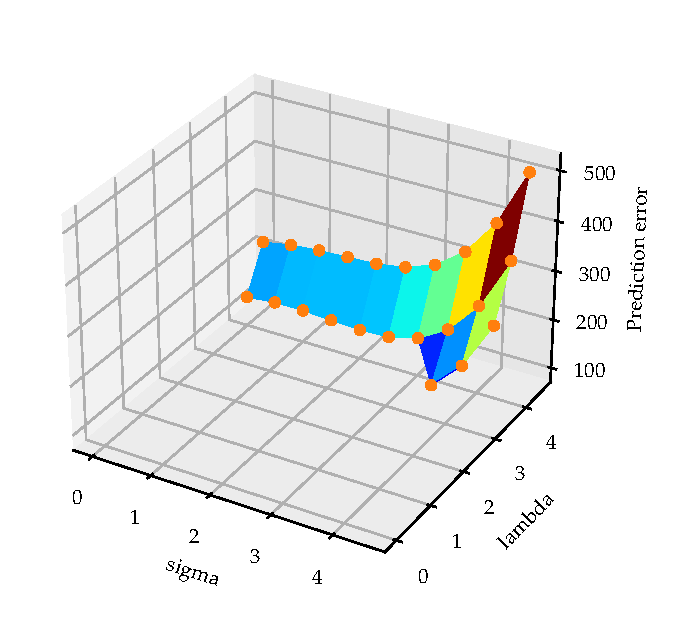
\includegraphics[width=0.9\textwidth]{Pictures/BO_vs_Grid2.eps}
%     \caption{Hyper parameter tuning of a model $M(\lambda, \sigma)$, 
%     35 evaluation in grid search vs 39 evaluations using Bayesian optimization}
%     \label{optimhist}
% \end{figure}
\begin{tcolorbox}[
    sharp corners,
    boxrule=0mm,
    enhanced,
    borderline west={4pt}{0pt}{gray},
    colframe=drGray,
    colback=drGray,
    coltitle=black,
]
{\large \textbf{Example: Bayesian Optimization}}\\
    Bayesian optimization is a \textit{probabilistic} surrogate-based optimization
    methodology. Here a cheap probabilistic regression model $p(y|x)$ is fitted to the
    the observations $\mathcal{D}$ and oppose to (deterministic) surrogate-based
    optimization, it is not possible right away to find the minima in the cheap
    surrogate model; first, we need to interpret the meaning of minima in a probabilistic
    regression model. This interpretation is done through a so-called acquisition
    function (more about this later). The policy is as following,
    $$\text{policy}_{BO}(\mathcal{D}) = \max_x AQ(p(y|x))$$
\end{tcolorbox}
\begin{figure}[H]%
    \centering
    {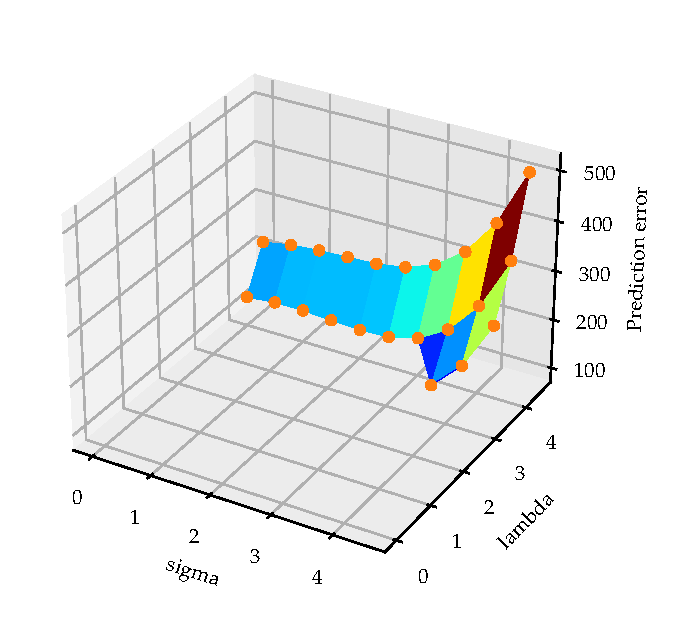
\includegraphics[width=0.46\textwidth]{Pictures/BO_vs_Grid2.eps} }%
    \qquad
   {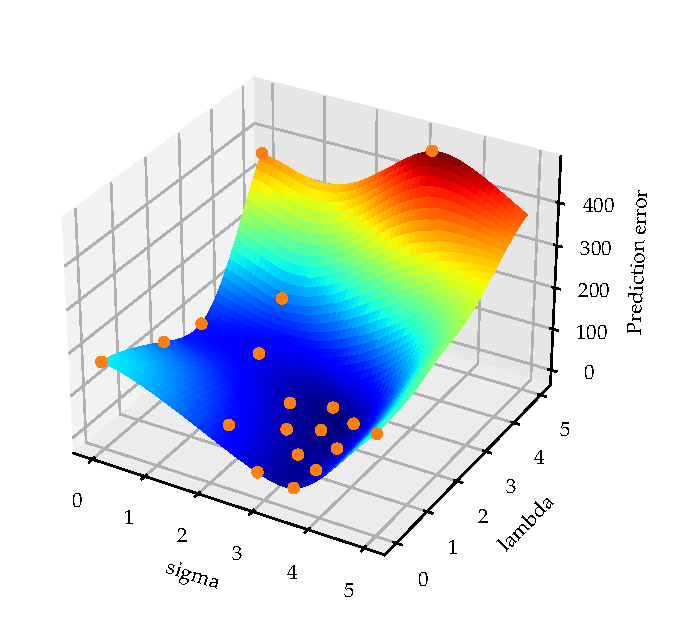
\includegraphics[width=0.46\textwidth]{Pictures/BO_vs_Grid1.eps} }%
    \caption{Hyper parameter tuning of a model $M(\lambda, \sigma)$, 
    23 evaluation in grid search vs 23 evaluations using Bayesian optimization}%
    \label{fig:example}%
\end{figure}


additionally, Bayesian Optimization allow for observation noise, 

\subsection{Observation model}\label{ObsModel}
Many optimization algorithms assume \textit{exact} evaluations of the objective function. However, this assumption
is often wrong especially for objective functions with real-life experiments, imperfect simulations, human interaction 
where measurement noise is a well known. The observation model is typically noisy and described as
$$y = f(x)+\epsilon$$ where $\epsilon$ is the measurement error, this is
typically assumed to be Gaussian with zero mean and a variance
$\sigma^2$ (which could depend on $x$ in a heterostodatic setting) and implies a Gaussian observation model, 
$$p(y|x,f(x),\sigma) = \mathcal{N}(y;f(x),\sigma^2)$$ 

% (note from now on we define $\phi := f(x)$ in order to avoid confusion and a extra set of paranteses)
% $$p(y|x,\phi,\sigma) = \mathcal{N}(y;\phi,\sigma^2)$$ 
we can extend this model to deal with noiseless observations as well, simply by setting $\sigma = 0$ and let the
model colaps into a Direct delta distribution, 
$$p(y|x, f(x)) = \mathcal{\delta}(y-f(x))$$
i.e. all probability mass for $y$ is on the value $f(x)$ giving the observation sample $y = f(x)$



\cleardoublepage

\chapter{Bayesian Optimization}
This chapter will introduce Bayesian optimization. We start with a general introduction to the
concept of optimization (mainly based on \cite{bayesoptbook}), which culminates with the
introduction of the idea of Bayesian optimization (BO). Next, we dive into the first BO component:
The Bayesian regression methodology. Finally, the concept of an acquisition function is introduced,
with a focus on expected improvement and a brief description of the other types. 

\section{Optimization methodology}
Given a cost/objective function $f: \mathcal{X} \rightarrow \mathbb{R}$, where the domain
$\mathcal{X}$ could be a subset of $\mathbb{R}^n$,
optimization is a methodology which seeks to find an optimal point, $x^*$, and value
$f^* = f(x)$, given as
\begin{align}\label{OPT}
    x^* \in \arg\min_{x \in \mathcal{X}} f(x) \hspace{1cm} f^* = \min_{x \in \mathcal{X}} f(x) = f(x^*).
\end{align}
Note that the above formulation is a minimization problem, which is equivalent to a
maximization problem maximizing $-f(\cdot)$. Throughout this thesis, we choose to only work
with a minimization problem. 
Solving this problem is intractable except for rare cases e.g. if $f$ is 
convex and analytically directly solvable or the domain of $f$ is very limited. Hm

\begin{testexample}[Direct solution method]
    The unconstrained linear least squares, $$\min_{x\in \mathbb{R}^n} f(x) := ||Ax-b||_2^2$$
    where $A \in \mathbb{R}^{m\times n}$ and $b \in \mathbb{R}^m$, is a convex problem,
    i.e. finding $x^*$ such that $\nabla f(x^*) = 0$ is equivalent to finding the solution
    to the problem. Assuming $A^TA$ is invertable, linear least squares can be solved
    directly by the normal equations, 
    $$\nabla f(x) = 2A^TAx + 2b^TA = 0 \hspace{0.5cm} \Leftrightarrow \hspace{0.5cm} x^* = (A^TA)^{-1} A^Tb$$
\end{testexample}

Most optimization problems are non-convex with multiple local minima. And even if the gradient is
given analytically the solution is found among a potentially infinitely large 
set of stationary points ($\nabla f(x) = 0$) and boundary points - this might be tedious or impossible.
When the problem is not directly solvable, mathematical optimization takes an indirect methodology: 
Design a sequence of experiments that reveal information of the objective function. This information 
can hopefully lead us to the solution of \eqref{OPT}. This general way of sequentially solving 
is presented in the book Bayesian Optimization by Roman Garnett \cite{bayesoptbook} and 
presented here as Algorithm \ref{algOPT}. 
W
\begin{algorithm}
\caption{Sequencial Optimization \cite{bayesoptbook} }\label{algOPT}
\begin{algorithmic}
\State \textbf{Input:} Initial dataset $\mathcal{D}$  \Comment{can be empty}
\While{Temination is not reached}
    \State $x \gets \text{policy}(\mathcal{D})$ \Comment{select next observation location}
    \State $y \gets \text{observe}(x)$ \Comment{observe objective function at chosen location}
    \State $\mathcal{D} \gets \mathcal{D} \cup \{(x,y)\} $ \Comment{update dataset}
\EndWhile
\State $\textbf{return: } \mathcal{D}$
\end{algorithmic}
\end{algorithm}

Given data points in the optimization landscape\footnote{"Optimization landscape" defined as the joint set of points in the domain and the objective function
evaluated in the points, i.e. $\{(x,f(x))\in \mathcal{X} \times \mathbb{R}| x \in \mathcal{X}\}$} 
a policy selects a point $x \in \mathcal{X}$ where we make our next observation. Policies can be deterministic or probibalitic, e.g. 
grid search and random search are examples of policies. The next observation provides us a $y$ value, which combined with $x$ is included to the 
available data $\mathcal{D}$. Finaly, a stopping criterion decides whether to continue or terminate. 

<example of random search is half as efficient as BO>


\begin{testexample}[Grid search]
    In grid search values along each dimention in $\mathcal{X}$ is seleced and combined with each
    other, which thereby defines a grid in the parameter space. All points are ordered and systematicly
    selected. In the content of algorhtim \ref{algOPT} we define the grid search policy as 
    $$\text{policy}_{GS}(\mathcal{D}) = x_{|\mathcal{D}|+1}$$
    assuming $x_1,x_2, \dots, x_{n}$ are the ordered grid points and the size of the obtained 
    data is $|\mathcal{D}|$. 
\end{testexample}
\begin{testexample}[Random search]
    In random search a uniform distribtuion is layed over the domain space $\mathcal{X}$ and a random point
    is selected from the distribtuion. 
    $$\text{policy}_{RS}(\mathcal{D}) = x, \hspace{0.5cm} x \sim p(\mathcal{X})$$
    Note that grid search and random search are policies which completely 
    ignores the available data. This is a shame and we can do better. 
\end{testexample}

\begin{testexample}[Gradient descent]
    Gradient descent is the most simple gradient-based optimization approach. The gradient of a continuous 
    function points in the most ascending direction from the location where it is evaluated.
    In the minimization task, \eqref{OPT}, we can iteratively use the opposite gradient direction, i.e. the most 
    descenting directiong. This yields the policy:
    $$\text{policy}_{GD}(\mathcal{D}) = x_n - \eta \nabla f(x_n)$$
    where we for a brief moment modify $y$ to be a vector, since the observation model 
    is given as:
    $$\text{observe}_{GD}(x) = [f(x), \nabla f(x)]$$
\end{testexample}

\begin{testexample}[Surrogate-based optimization]
    <SVR> <Radial Basis function> <Polynomal model/respons surface>
    In surrogate-based optimization all available data is fitted by a cheap-to-evaluate approximation
    to the objective function - this approximation is called a \textit{surrogate} model. Examples
    of surrogate models could be a neural network or a random forest. The next point is 
    chosen as the point where the surrogate model is minimized. 
    $$\text{policy}_{sur}(\mathcal{D}) = \min_x \hat f(x)$$
    where $\hat f(x) \approx f(x)$ for $x$ close to the data $\mathcal{D}$. And we hope the approximation
    holds for $x$ far away from the the data. \textbf{}
\end{testexample}

\subsection{When to use Bayesian optmization}
What if $f(x)$ took serval days to evaluate. What if $f(x)$ is noisy? what if discrete points? 
<more here>

% \begin{figure}[h]
%     \centering
%     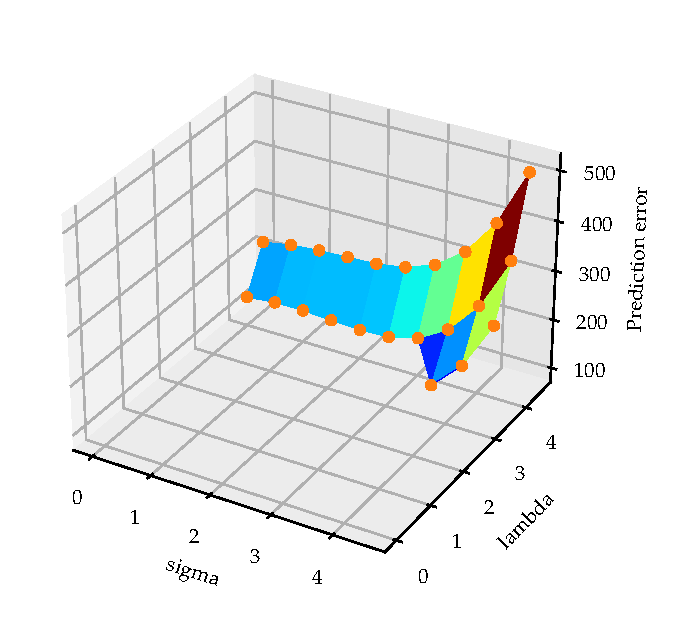
\includegraphics[width=0.9\textwidth]{Pictures/BO_vs_Grid2.eps}
%     \caption{Hyper parameter tuning of a model $M(\lambda, \sigma)$, 
%     35 evaluation in grid search vs 39 evaluations using Bayesian optimization}
%     \label{optimhist}
% \end{figure}
\begin{tcolorbox}[
    sharp corners,
    boxrule=0mm,
    enhanced,
    borderline west={4pt}{0pt}{gray},
    colframe=drGray,
    colback=drGray,
    coltitle=black,
]
{\large \textbf{Example: Bayesian Optimization}}\\
    Bayesian optimization is a \textit{probabilistic} surrogate-based optimization
    methodology. Here a cheap probabilistic regression model $p(y|x)$ is fitted to the
    the observations $\mathcal{D}$ and oppose to (deterministic) surrogate-based
    optimization, it is not possible right away to find the minima in the cheap
    surrogate model; first, we need to interpret the meaning of minima in a probabilistic
    regression model. This interpretation is done through a so-called acquisition
    function (more about this later). The policy is as following,
    $$\text{policy}_{BO}(\mathcal{D}) = \max_x AQ(p(y|x))$$
\end{tcolorbox}
\begin{figure}[H]%
    \centering
    {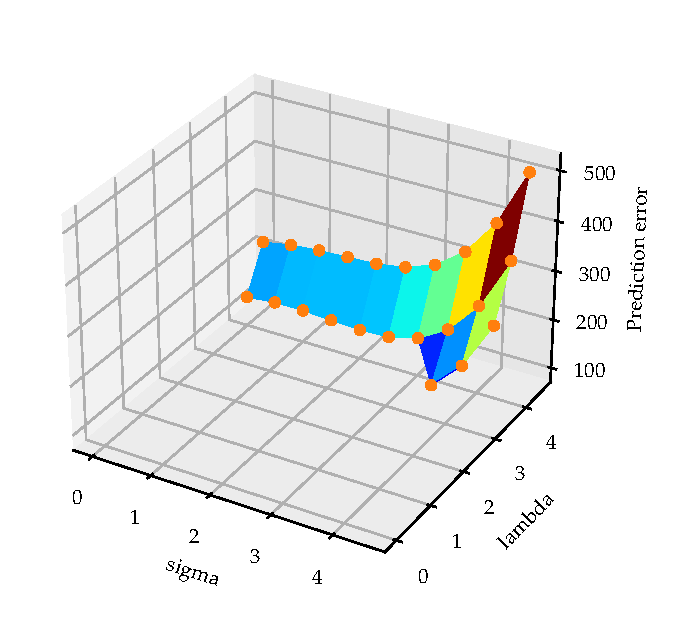
\includegraphics[width=0.46\textwidth]{Pictures/BO_vs_Grid2.eps} }%
    \qquad
   {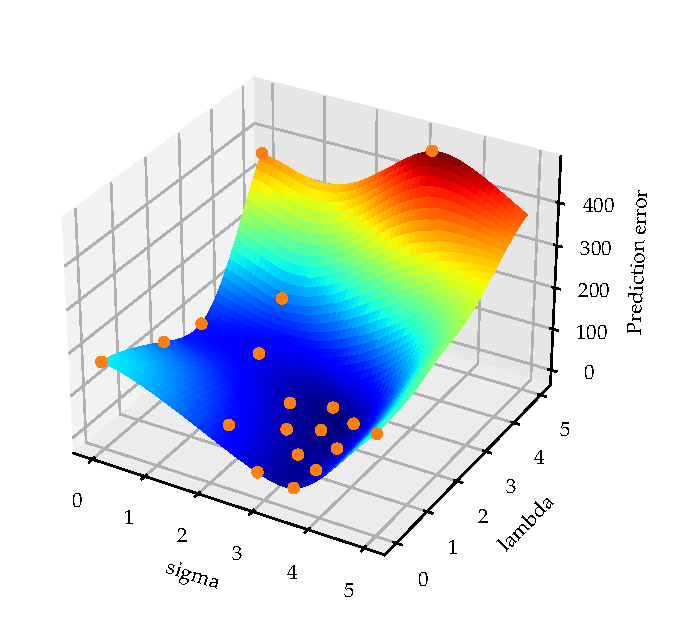
\includegraphics[width=0.46\textwidth]{Pictures/BO_vs_Grid1.eps} }%
    \caption{Hyper parameter tuning of a model $M(\lambda, \sigma)$, 
    23 evaluation in grid search vs 23 evaluations using Bayesian optimization}%
    \label{fig:example}%
\end{figure}


additionally, Bayesian Optimization allow for observation noise, 

\subsection{Observation model}\label{ObsModel}
Many optimization algorithms assume \textit{exact} evaluations of the objective function. However, this assumption
is often wrong especially for objective functions with real-life experiments, imperfect simulations, human interaction 
where measurement noise is a well known. The observation model is typically noisy and described as
$$y = f(x)+\epsilon$$ where $\epsilon$ is the measurement error, this is
typically assumed to be Gaussian with zero mean and a variance
$\sigma^2$ (which could depend on $x$ in a heterostodatic setting) and implies a Gaussian observation model, 
$$p(y|x,f(x),\sigma) = \mathcal{N}(y;f(x),\sigma^2)$$ 

% (note from now on we define $\phi := f(x)$ in order to avoid confusion and a extra set of paranteses)
% $$p(y|x,\phi,\sigma) = \mathcal{N}(y;\phi,\sigma^2)$$ 
we can extend this model to deal with noiseless observations as well, simply by setting $\sigma = 0$ and let the
model colaps into a Direct delta distribution, 
$$p(y|x, f(x)) = \mathcal{\delta}(y-f(x))$$
i.e. all probability mass for $y$ is on the value $f(x)$ giving the observation sample $y = f(x)$




% <Cope with inacuracies> i.e. allows for stochastic objective function. 
% <Uncertainty measure with prediction based on simple and clear prior 
% assumptions about the characteristic about the objective function. >
% <Provides an adequate termination condition for the opt. process>. 

% <kilde 151. Bayes Opt is assumed superior to other global optimization technics 
% with limited budget>

\section{Bayesian regression}
Whereas traditional regression workflow is the following: Given data, choose the best fitting model
parameters, make predictions using those parameters. The Bayesian framework allows us to skip the
dependency of a single set of parameters and instead use \textit{all possible} parameters by treating the set
of parameters as a random quantity, $\theta \sim p(\theta|\mathcal{D})$, where some values/realizations of $\theta$ are more
probable than others given data. In Bayesian regression we are interest is the predictive posterior distribution,  
\begin{align}\label{Predictive2}
    p(y|x, \mathcal{D}) &= \int p(y,\theta|x, \mathcal{D}) d\theta\\
    &= \int p(y|x,\theta)p(\theta|\mathcal{D}) d\theta,
\end{align}
where the posterior $p(\theta|\mathcal{D})$ gives weighting to the proposed regression model
$p(y|x,\theta)$. Note that the second equation is true because of the probability chain rule and
that $y$ is fully described by the parametric model $p(y|x,\theta)$ and the parameters $\theta$ are
fully described by the posterior distribution $p(\theta|\mathcal{D})$.
\begin{testexample2}[Bayesian methodology]
    In Bayesian modelling $p(\theta|\mathcal{D})$ is the posterior distribution, and it is linked
     to the likelihood $p(\mathcal{D}|\theta)$ and prior $p(\theta)$ via Bayes rule,
    $$p(\theta|\mathcal{D}) = \frac{p(\mathcal{D}|\theta)p(\theta)}{p(\mathcal{D})} \propto p(\mathcal{D}|\theta)p(\theta),$$
    where the approximation holds since $p(\theta|\mathcal{D})$ is only a function of $\theta$. 
    In the case of regression, we always condition on $\textbf{x}$, i.e. $\mathcal{D} = \textbf{y}|\textbf{x}$, 
    more concretely we write, 
    $$p(\theta| \mathcal{D}) = \frac{p(\textbf{y}|\textbf{x}, \theta)p(\theta|
    \textbf{x})}{p(\textbf{y}|\textbf{x})} \propto p(\textbf{y}|\textbf{x}, \theta)p(\theta| \textbf{x})$$
    The modeling task to is to specify a likelihood $p(\textbf{y}|\textbf{x},\theta)$, which encodes how likely the model $\theta$
    explian the data, and a prior $p(\theta|\textbf{x})$, which encodes our prior belief about the model. 
\end{testexample2}

\subsection{Surrogate model}
A surrogate model in a Bayesian optimization setting is a Bayesian regression model. The most
used surrogate model is a Gaussian Process. But there have been investigations on other 
surrogates, such as Bayesian neural networks and Bayesian regression trees. These are all
discriminative models, and another approach we focus on in this project is to model $y$ and
$x$ jointly in a so-called generative model, $p(x,y)$. A generative model can be used implicitly
as a surrogate from the conditional distribution of $y$ given $x$, $p(y|x)$.

In this thesis, the Bayesian regression models investigated as Bayesian optimization surrogates are
the following:
\begin{itemize}[noitemsep]
    \item Gaussian process (GP)
    \item Bayesian neural network (BNN)
    \item Kernel density regression (KDE)
    \item Gaussian mixture regression (GMR)
    \item Sum-product networks (SPN)
\end{itemize}

We now introduce the concept of inference, which is necessary for using the probabilistic surrogate models
in Bayesian Optimization. 

\subsection{Inference of surrogate models}
Inference is the process of computing answers to queries about a probabilistic model after observing
data. In Bayesian regression, the query is the predictive distribution, $p(y|x,\mathcal{D})$, as we
are interested in the distribution of $y$ given $x$ and already observed data, $\mathcal{D}$. This
often indirectly create the posterior query, $p(\theta|\mathcal{D})$, the probability of model
parameters $\theta$ given data $\mathcal{D}$. Lastly, it is also inference when we train a Gaussian
mixture model or SPN using the expectation-maximization algorithm (EM) since we are iteratively
answering the query $E_{p(z|\theta^{(k)})}[z|\theta]$.

%\subsection{Exact and approximate inference}
We distinguish between two different ways of inference: Exact and approximate inference. It is
\textit{exact inference} when a probabilistic query is calculated exact. It is possible to
calculate exact inference on the predictive distribution for the Gaussian mixture model, Sum product
network, and Gaussian processes. Models which allow for exact inference have a powerful advantage
over the models with approximate inference since we can guarantee the answers to the queries are
correct; however, they are usually also less expressive (unable to explain complicated models). 

When it is not possible to answer a probabilistic query exact, we can approximate the answer using
\textit{approximate inference}. When dealing with complicated and expressive statistical models,
exact inference is often intractable, and we need to use approximate inference. Approximate
inference is a broad category of methods, which includes variational inference and Markov chain
Monte Carlo (MCMC). The two Bayesian Neural networks, we deal with in this project, Bohamiann and
Numpyro BNN are similar regression models but are inferred using two different MCMC methods,
Hamiltonian Monte Carlo - giving different results. As revealed later (see in section \ref{BNN})
approximate inference might be flawed and inexact. 

\begin{table}[H]
    \centering
    \begin{tabular}{l|l|l}
    %\rowcolor[HTML]{C0C0C0} 
    \textbf{Model}       & \textbf{Predictive inference}    &   \textbf{Learning} \\ \hline
    GP                          & Exact $O(n^3)$            & Emperical Bayes\\
    Numpyro BNN                 & No U-Turn Sampler         & \\
    Bohamiann BNN               & Adaptive stochatic HMC    & \\
    Kernel density regression   & Exact $O(n)$              & \\
    Gaussian mixture regression & Exact $O(K)$              & EM  \\
    SPN                         & Exact $O(E)$              &  EM $O(E)$\\
    \end{tabular}
    \caption{Overview of inference methods applied on the statistical models used in this project.
            $E$ is the number of edges in the SPN. $n$ is the number of data points. $K \leq n$ is
            the number of mixture components. We will soon learn that for an SPN the number of
            mixture components is exponentially larger than the number of edges i.e. $E << K$. In theory
            MCMC methods samples from true the posterior distribution, and do not need any
            fitting/learning. }
\end{table}

\newpage
\section{Acquisition function}
Given a correct predictive distribution $p(y|x\mathcal{D})$ the next step in Bayesian optimization
is to select the next location $x \in \mathcal{X}$ to sample from. The next location is chosen
according to a so-called acquisition function (AQ function), which balances out the well-known
concept of exploitation and exploration. It is exploitation if the next chosen location according to
its average improvement. It is exploration if the next point is chosen in a region of high
uncertainty and thereby helps lower the overall uncertainty. First, we will look at the acquisition
function used in the thesis: Expected improvement. Secondly, we shortly present other different
types of acquisition functions. In Figure \ref{Different_AQ_functions} we see three different
acquisition functions. The expected improvement (EI) is known for being biased towards exploitation.
In contrast, the negative lower confidence bound (LCB) has a parameter $\beta$, which can be tuned
to make it focus more on exploration. 
\begin{figure}[H]
    \centering
    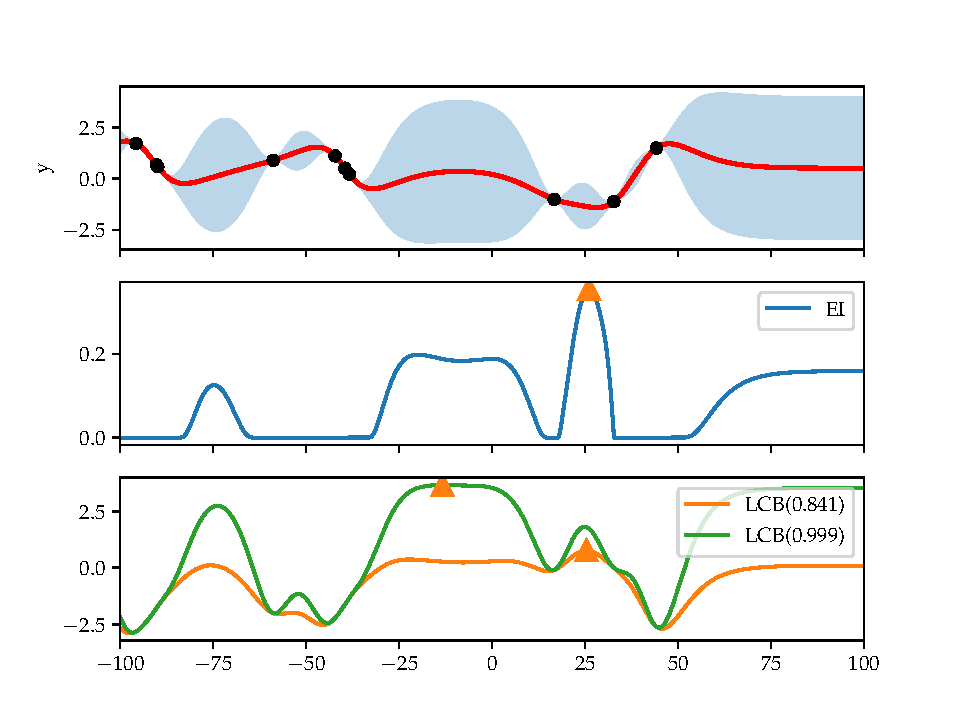
\includegraphics[trim=1cm 0cm 1cm 1cm,clip,width=\textwidth]{Pictures/illustration_AQs.pdf}
    \caption{The same regression model and points as Figure \ref{BO_example}, but with three
    different acquisition functions: Expected improvement and negative lower confidence bound for
    two different lower quantiles $0.841$ and $0.999$. The latter yields more exploration.}\label{Different_AQ_functions}
\end{figure}

\begin{figure}[H]
    \centering
    \begin{minipage}[b]{0.32\textwidth}
      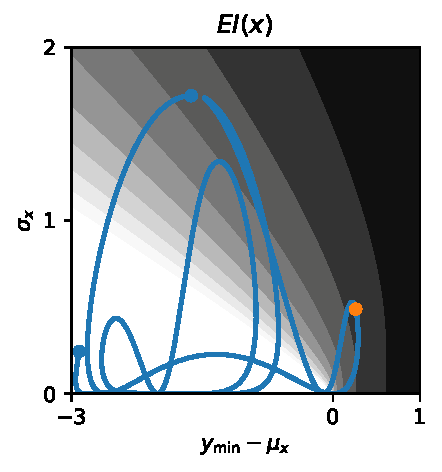
\includegraphics[trim=0.2cm 0.2cm 0cm 0.1cm,clip,width=\textwidth]{Pictures/expected_improvement_illustration.pdf}
    \end{minipage}
    \hfill
    \begin{minipage}[b]{0.32\textwidth}
        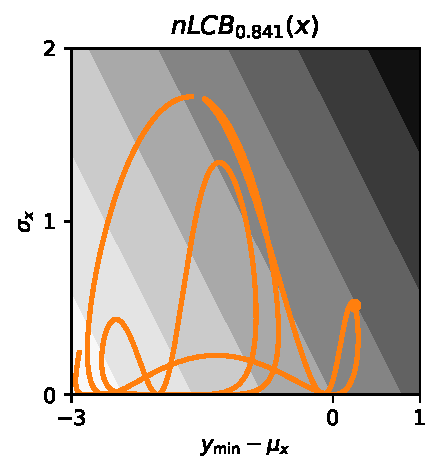
\includegraphics[trim=0.2cm 0.2cm 0cm 0.1cm,clip,width=\textwidth]{Pictures/neg_lower_confidence_illustration_1.pdf}
      \end{minipage}
     \hfill
     \begin{minipage}[b]{0.32\textwidth}
        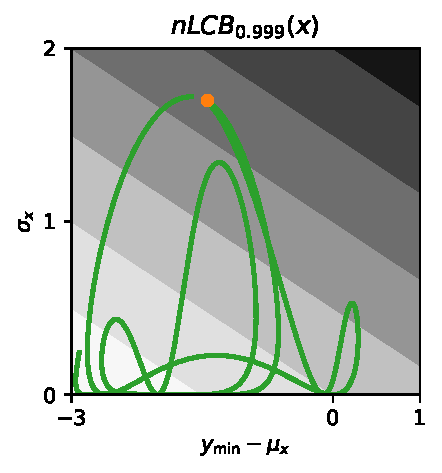
\includegraphics[trim=0.2cm 0.2cm 0cm 0.1cm,clip,width=\textwidth]{Pictures/neg_lower_confidence_illustration_3.pdf}
      \end{minipage}
    \caption{Contourplot of expected improvement (EI) and lower confidence bound (LCB) for two different
    quantiles for different (Gaussian) predictive uncertainties $\sigma_x =
    \sqrt{\mathbb{V}ar_{p(y|x,\mathcal{D})y]}}$ versus the average improvement $y_{\min}-\mu_x$,
    where $\mu_x = E_{p(y|x,\mathcal{D})}[y]$. Darker colors indicates higher values. The colored lines are the
    mapping $x \mapsto (\sigma_x, y_{\min}-\mu_x)$ for $x = [-100, 100]$ for the Bayesian regression
    function in Figure \ref{Different_AQ_functions} - and thereby explains how the acquisition
    functions balances exploitation and exploration. The orange dot represent the point maximizing
    the acquisition function}
    \label{EI_illustration}
\end{figure}


\subsection{Expected improvement}
A popular choice of acquisition function is expected improvement, 
$$EI(x) = \mathbb{E}_{p(y|x,\mathcal{D})}[\max(0, y_{\min}-y)]$$ where we only consider the values
$y$, which improves the current best value in the expectation of the predictive distribution,
$p(y|x,\mathcal{D})$. Therefore, a $x$ which yield a bad predictive mean value
$\mathbb{E}_{p(y|x,\mathcal{D})}[y]> y_{\min}$ might still be maximizing the expectated improvement,
if the predictive uncertainty is very large at $x$. Figure \ref{EI_illustration} illustrates that a
large uncertainty in the predictive distribution (represented as the predictive variance) can lead
to relative large values even for non-improving mean predictions.


\begin{note2}[Why defining expected improvment with max]    
    Note that $\max(0,\cdot)$ is important since the Bayesian optimization othervise reduces to
    a simple non-probabilistic surrogate-based optimization method,
    \begin{align*}
        \mathbb{E}_{p(y|x,\mathcal{D})}[y_{\min}-y] = y_{\min} - \mathbb{E}_{p(y|x,\mathcal{D})}[y]
    \end{align*}
    i.e. maximizing the above is equivalent to maximizing the predictive mean, and thereby we loose
    all the valuable information about the predictive uncertainties from the Bayesian regression model. 
\end{note2}

\subsubsection{Exact expected improvement} \label{ExactEI} 
In the following derivation we assume the
predictive distribution can be approxiamted by a normal distribution dependent on the point of
interest $x$ and the data $\mathcal{D}$ (note for the GP it is in fact not an approximation), 
$$p(y|x,\mathcal{D}) \approx \mathcal{N}(y|\mu(x,\mathcal{D}), \sigma^2(x,\mathcal{D}))$$ where we
will change to a less clumpsy notation $\mathcal{N}(y|\mu_x,
\sigma^2_x):=\mathcal{N}(y|\mu(x,\mathcal{D}), \sigma^2(x,\mathcal{D}))$. This is completely fine
since we $x$ is fixed (and $\mathcal{D}$ is fixed) when evaluating the expected improvement in a point
$x$. %  $\sigma_x := \sigma^2(x,\mathcal{D})$ and $\mu_x := \mu(x,\mathcal{D})$
%as evaluated functions, i.e. numbers. 
Furthermore, the density of
a standard normal distribution is denoted $\phi(\cdot):=\mathcal{N}(\cdot | 0,1)$, and the cumlative
density function (CDF) of a standard normal distribution is denoted, $\Phi(\cdot) :=
\int_{-\infty}^{\cdot} \phi(\epsilon)d\epsilon$. We will now see that the normal approximation
of the predictive distribution yiels closed form solution to the expected improvement function, 

\begin{align*}
    E_{\mathcal{N}(y|\mu_x, \sigma_x^2)}[\max(0,y_{\min}-y)] &= \int \max(0,y_{\min}-y) \mathcal{N}(y|\mu_x, \sigma_x^2) dy\\
    &= \int_{-\infty}^{y_{\min}} (y_{\min}-y) \frac{1}{\sigma_x}\phi\left(\frac{y-\mu_x}{\sigma_x}\right) dy\\
    &= \int_{-\infty}^{\frac{y_{\min}-\mu_x}{\sigma_x}} (y_{\min}-\mu_x-\sigma_x\epsilon) \frac{1}{\sigma_x}\phi\left(\epsilon\right) \sigma_x d\epsilon\\
    &= \int_{-\infty}^u \sigma_x \cdot (u-\epsilon) \phi(\epsilon) d\epsilon\\
    &=  \sigma_x \cdot \left( u\cdot \int_{-\infty}^u \phi(\epsilon) d\epsilon +\int_{-\infty}^u (-\epsilon)  \phi(\epsilon) d\epsilon \right) \\
    &= \sigma_x [u\Phi(u)+ \phi(u)]
\end{align*}

where $u:=\frac{y_{\min}-\mu_x}{\sigma_x}$. 

\begin{note2}[Derivation details]
    To understand the identity $\phi(u) = \int_{-\infty}^u
    (-\epsilon)  \phi(\epsilon) d\epsilon$ used in the last equality, we first see that the antiderivative
is $\phi(\epsilon) = \frac{1}{\sqrt{2\pi}} \exp\left(\frac{-\epsilon^2}{2}\right)$,
\begin{align*}
    \frac{d}{d \epsilon} \phi(\epsilon) =  \frac{1}{\sqrt{2\pi}}\frac{d}{d \epsilon}  \exp\left(\frac{-\epsilon^2}{2}\right) 
    =  \frac{1}{\sqrt{2\pi}}\exp\left(\frac{-\epsilon^2}{2}\right)(-\epsilon)
    = -\epsilon \phi(\epsilon)
\end{align*}
and evaluating the rieman integral is equivalent to evaluate the antiderivative in its boundaries, giving the 
solution, 
$$\int_{-\infty}^u
(-\epsilon)  \phi(\epsilon) d\epsilon = \left[\phi(\epsilon)\right]_{-\infty}^u = \phi(u)-0 = \phi(u)$$ 
\end{note2}

We can also explicily write the expected improvement as, 
$$EI(x) = (y_{\min}-\mu_x)\Phi\left(\frac{y_{\min}-\mu_x}{\sigma_x}\right)+ \sigma_x
\phi\left(\frac{y_{\min}-\mu_x}{\sigma_x}\right)$$ where the first part can be interpretted as
exploitation (favouring points with a large average improvement $I(x) := (y_{\min}-\mu_x)$) and the second
part can be seen a exploitation (favouring points with high uncertainty.). This can also be seen
in Figure \eqref{EI_illustration}, where it is clear that the expected improvement is growing for
growing average improvement $I(x)$ and also for growing prediction uncertainty $\sigma_x$.


% taking the derivative with
% respect to $I(x) := (y_{\min}-\mu_x)$ and $\sigma_x$, we see that expected improvement is is
% increasing if the improvement grows or if the variance $\sigma_x$ grows, i.e
% $$\frac{\partial EI(x)}{\partial I(x)} = \Phi\left(\frac{y_{\min}-\mu_x}{\sigma_x}\right) > 0, \hspace*{0.5cm} 
% \frac{\partial EI(x)}{\partial \sigma_x} = \phi\left(\frac{y_{\min}-\mu_x}{\sigma_x}\right) >0$$ 
% <obs mistake in the book!!!?>

\subsubsection{Approximate expected improvement}
If the predictive distribution is non-Gaussian, it is either possible to approximate it as a Gaussian
(By using the mean and variance of the predictive distribution to define the Gaussian approximation)
or calculate the expected improvement approximately as follows, 
\begin{align*}
    E_{p(y|x,\mathcal{D})}[\max(0,y_{\min}-y)] &= \int \max(0,y_{\min}-y) p(y|x,\mathcal{D}) dy\\
    &\approx \frac{1}{K} \sum_{k=1}^K  \max(0,y_{\min}-y^{(k)})
\end{align*}
where $y^{(k)}$ are samples from the predictive distribution.

% In the case of a parametric model
% like a Bayesian NN, then we already got posterior samples from posterior $\theta^{(k)} \sim p(\theta | \mathcal{D})$, giving, 
% $$p(y|x,\mathcal{D}) \approx \frac{1}{K_2} \sum_{k=1}^{K_2} p(y|x,\theta^{(k)})$$ where
% $p(y|x,\mathcal{D} = \mathcal{N}(y|NN_w,\sigma))$. So essentially we should sample from a sampled
% distribution, but instead the PhD thesis \cite{PhDthesis}, just sample the mean and set $K_2 = 1$... 


% \begin{align*}
%     \mathbb{E}_{y_*|\textbf{x}_*,D_n}[\max(0,y_{\min}-y_*)] &= ??\\
%     \mathbb{E}[\min(0,y_{\min}-y_*)|\textbf{x}_*,D_n] &= \int_{-\infty}^\infty \min(0,y_{\min}-y_*) p(y_*|\textbf{x}_*,D_n) dy_*\\
%     &= \int_{-\infty}^{y_{\min}} (y_{\min}-y_*) p(y_*|\textbf{x}_*,D_n) dy_*\\
%     &\approx \frac{1}{N} \sum_{\theta \in \Omega } [y_{\min}-f_\theta(x)]
% \end{align*}

% where $\Omega = \{\theta|f_{\theta}(x)< y_{\min}\}$

%\section{uncertainties}
%Alatoric vs epistemic uncertainties 
\subsection{Other acquisition functions}
Expected improvement is just one choice of acquisition function, we now shortly present three different acquisition functions, 
Lower confidence bound, entropy search (mutual information acquisition) and probability of improvement. As mentioned, we
only use expected improvement in this thesis.

\subsubsection{Lower confidence bound}
Lower confidence bound acquisition function \cite[145]{bayesoptbook}\footnote{
\cite[145]{bayesoptbook} deals with an maximization problem, and an upper confidence bound
acquisition function is presented, however, this formulation is equivalent.} is parameterised by a
confidence parameter $\pi \in [0,1]$ which defines the preditive $(1-\pi)$-quantile at $x$,
 $$q_{1-\pi}(x) = \inf \{y^*|\mathbb{P}(y\leq y^* | x, \mathcal{D}) \geq (1-\pi) \},$$
i.e. the prediction $y \sim p(y|x, \mathcal{D})$ will only be be less than the lower bound $q_{1-\pi}(x) $
with a tunable probability of $1-\pi$. 
The acquisition function is simply defined as the negative lower quantile
$$LCB_{\pi}(x) = -q_{1-\pi}(x).$$ It is negative since we want to find the next location which
maximizes the acquisition function. Choosing a confidence level close to 1, i.e. $\pi \approx 1$ yields
exploration, as seen in figure \ref{Different_AQ_functions}. For a Gaussian predictive distribution
this the lower confidence bound is simply given as, 
$$LCB(x) = - (\mu_x - \beta \sigma_x)$$
where $\beta = \Phi^{-1}(\pi)$. 
% \begin{figure}[H]
%     \centering
%     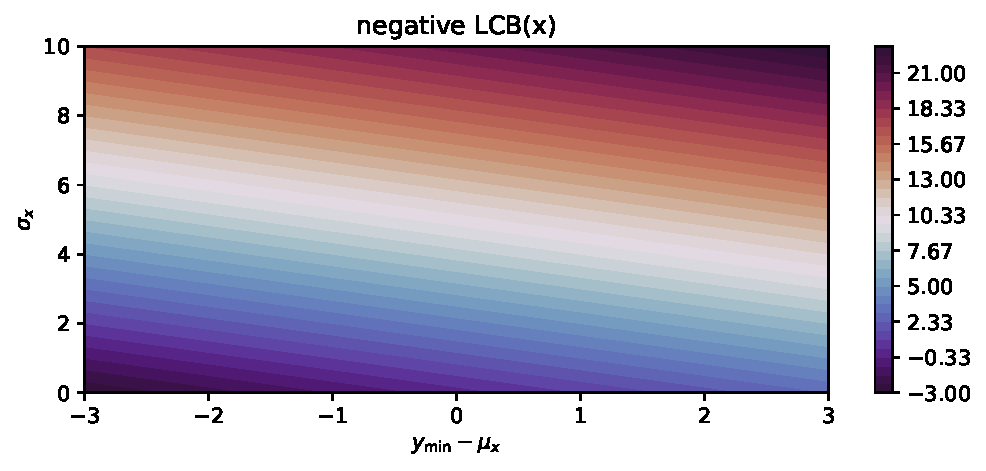
\includegraphics[width=\textwidth]{Pictures/neg_lower_confidence_illustration.pdf}
%     \caption{<Soon similar plot as Figure \ref{EI_illustration}> Illustration of the values of the
%     negative lower confidence bound for different predictive uncertainties $\sigma_x =
%     \sqrt{\mathbb{V}ar_{p(y|x,\mathcal{D})}[y]}$ versus the average improvement $y_{\min}-\mu_x$,
%     where $\mu_x = E_{p(y|x,\mathcal{D})}[y]$}
%     \label{nLCB_illustration}
% \end{figure}

\subsubsection{Entropy search}
Optimization policies known as policy search utilize information theory to select the next point
which will provide the most information (i.e useful knowledge) about the objective function. 
More specifically their acquisition function is \textit{mutual information} \cite[135-140]{bayesoptbook}, 
\begin{equation}\label{mutualinfo}
    I(x,y) = \int \int p(x,y) \log \frac{p(x,y)}{p(y)p(x)} dy dx,
\end{equation}
which is a measurement of dependency between the random variables. If $x$ and $y$ are independent, then
$p(x,y) = p(x)p(y)$, i.e. the fraction in \eqref{mutualinfo} becomes 1 and thereby $I(x,y) = 0$. 



% uncertainty about the objective function over a larger volume. Expected
% improvement (gure 7.3) and probability of improvement (gure 7.9),
% on the other hand, are computed only from inspection of the marginal
% predictive distribution 𝑝(𝑦 | 𝑥, D). As a result, they cannot dierentiate
% observation locations based on their global impact on our belief.


% The reasoning underlying entropy search policies is somewhat different from and more general than the other acquisition functions we
% have considered thus far, all of which ultimately focus on maximizing
% the posterior mean function. Although this is a pragmatic concern, it is
% information-theoretic decision making as a intimately linked to optimization. Information-theoretic experimental
% model of the scientic method design is instead motivated by an abstract pursuit of knowledge, and may
% be interpreted as a mathematical formulation of the scientic method.

%One-step lookahead with (either) information gain yields an acquisi function known as mutual
%information



\subsubsection{Probability of improvement}
Probability of improvment acquisitionfunction is defined as follows, 
$$PI(x) = \mathbb{P}{p(y|x,\mathcal{D})}(\max(0,y_{\min}-y)>0) =
\mathbb{P}{p(y|x,\mathcal{D})}(y<y_{\min})$$ i.e. the probability of the prediction is an actually
improvement. It does not take the magnitude of the improvement into consideration (as Expected
improvement). It rather just if there is an improvement or not. In the case of a Gaussian predictive
probability it is given on closed form
$$PI(x) = \Phi·\left(\frac{y_{\min}-\mu_x}{\sigma_x}\right)$$
where $p(y|x\mathcal{D}) =\mathcal{N}(y|\mu_x,\sigma_x^2) =\mu_x + \sigma_x\cdot\mathcal{N}(y|0,1)$

% We then discuss the knowledge
% gradient (Section 4.2), entropy search, and predictive entropy search (Section 4.3) acquisition functions.
% These alternate acquisition functions are most useful in exotic problems where an assumption made by
% expected improvement that the primary benefit of sampling occurs through an improvement at the point
% sampled is no longer true.


% The entropy search (ES) (Hennig and Schuler, 2012) acquisition function values the information we have
% about the location of the global maximum according to its differential entropy

% ES seeks the point to evaluate what causes the largest decrease in differential entropy

% (Recall from, e.g., Cover and Thomas (2012),
% that the differential entropy of a continuous probability distribution p(x) is R
% p(x) log(p(x)) dx, and that
% smaller differential entropy indicates less uncertainty.)

% Predictive entropy search (PES) (Hern´andezLobato et al., 2014) seeks the same point but uses a reformulation of the entropy reduction objective
% based on mutual information. Exact calculations of PES and ES would give equivalent acquisition functions, but exact calculation is not typically possible, and so the difference in computational techniques
% used to approximate the PES and ES acquisition functions creates practical differences in the sampling
% decisions that result from the two approaches. We first discuss ES and then PES.

% Let x  be the global optimum of f. The posterior distribution on f at time n induces a probability
% distribution for x
% . Indeed, if domain A were finite, we could represent f over its domain by a
% vector (f(x): x ∈ A), and x
% would correspond to the largest element in this vector. The distribution of
% this vector under the time-n posterior distribution would be multivariate normal, and this multivariate
% normal distribution would imply the distribution of x

% . When A is continuous, the same ideas apply,
% where x

% is a random variable whose distribution is implied by the Gaussian process posterior on f




% With kriging, we can develop search methods that put some emphasis on sampling where the standard
% error is high. In this way, we obtain the desired feature of ‘paying attention to parts of the space
% that have been relatively unexplored.’
\cleardoublepage

\chapter{Bayesian regression models - probabilistic surrogate model}
As mentioned in the previous sections, the first of two repeated steps in Bayesian optimization
is to create a good Bayesian regression model. %why not non bayesian regression? 
i.e. finding the probility of prediction for a arbitrary point $x$ given datapoints 
$\mathcal{D} = \{x_1, y_1, \dots, x_n, y_n\}$, 
 $$p(y|x,\mathcal{D})$$

The surrogate model of choise in Bayesian optimization is a Gaussian Process, and Bayesian Neural Network.
These are discriminative models, however, another approach, which we focus on in this project, is
to model $y$ and $x$ jointly in a so-called generative model.

\section{Gaussian mixture regression}
Taking a convex combination of a set of multivariate Gaussian distributions is a Gaussian mixture model
$$p(z) = \sum_{k=1}^K \pi_k \mathcal{N}(z|\mu_k, \Sigma_k)$$  
Defining $z := (x,y)$ we can model our data, as a generative model $p(x,y)$, now, since the conditonal 
of a Gaussain mixture again is Gaussain mixture - i.e. closed form expression, we can exactly calculate
$p(y|x) = GMM_{y|x}$

Assuming iid data the likelihood is given as 
$$p(\mathcal{D}|\mu_1, \dots, \mu_K, \Sigma_1, \dots, \Sigma_K, \pi_1, \dots, \pi_K) = \prod_{i=1}^n \sum_{k=1}^K \pi_k \mathcal{N}(z_i|\mu_k, \Sigma_k)$$
And the log likelihood, 
$$\log p(\mathcal{D}| ..) = \sum_{i=1}^n \log \sum_{k=1}^K \pi_k \mathcal{N}(z_i|\mu_k, \Sigma_k)$$


\subsection*{Dealing with wrong variance}
\begin{figure}[H]%
    \centering
    {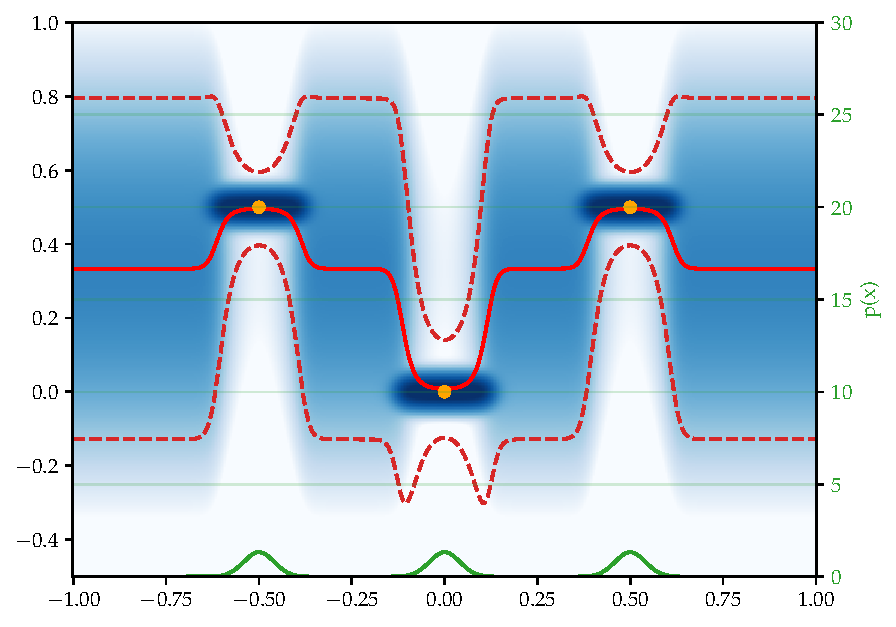
\includegraphics[width=0.46\textwidth]{Pictures/mixture_regression_variance_problem1.pdf} }%
    \qquad
   {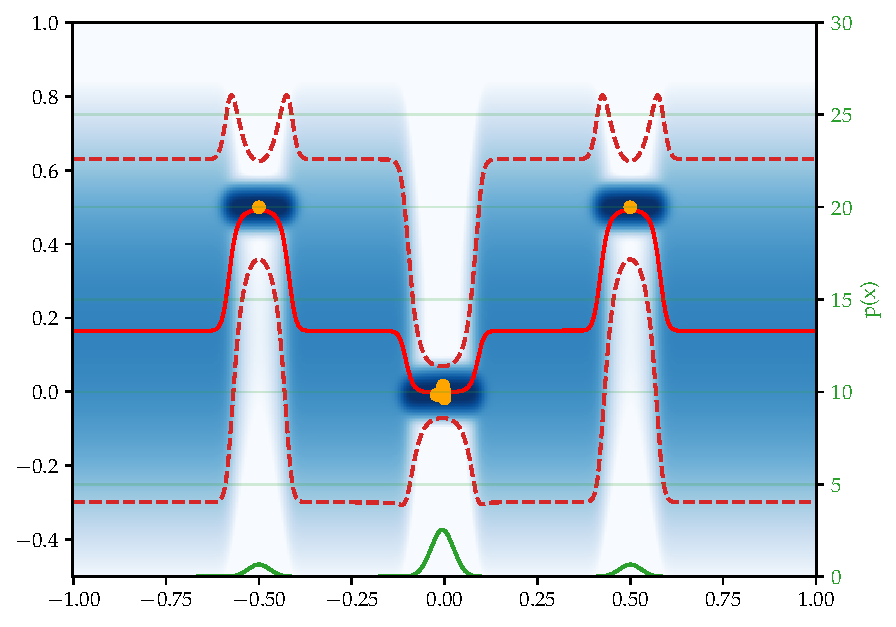
\includegraphics[width=0.46\textwidth]{Pictures/mixture_regression_variance_problem2.pdf} }%
   \qquad
   {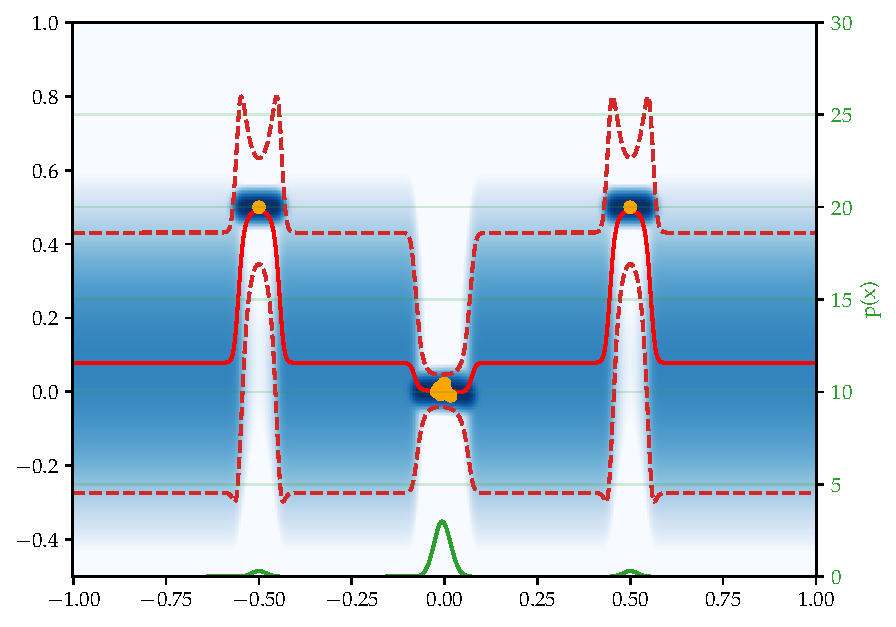
\includegraphics[width=0.46\textwidth]{Pictures/mixture_regression_variance_problem3.pdf} }%
   \caption{EI improvement might in this case be stucked at the point 0,
    since the conditional distribution is normalized by $p(x)$ and therefore not
    influenced by the amount of data}%
    \label{MixtureReg_challenge}%
\end{figure}


<variance manipulation>
<Expected improvement manipulation>


\section{Mixture regression in a Bayesian setting}
As seen in examples. The uncertainty of conditional distribution is way too certain
in areas with no data points, therefore we need to enhance the model with some bayesian 
flavour. 

$$p(y|x,\mathcal{D}) = p(y|x,Z)p(Z|x)$$



\subsection*{Expetation-maximization algorithm}
A way to find local maxima in the likehood function is using the EM algorithm. 

If we define a latent/hiddem random variabel $Z_i \in \{1,\dots, K\}$ for each data point, then 
the likelihood function becomes, 
$$L(\theta|\mathcal{D}, Z) = \prod_{i=1}^n \sum_{k=1}^K 1(Z_i = k) \pi_k \mathcal{N}(z_i|\mu_k, \Sigma_k)$$

Now the expectation wrt. the current value $p(Z|\mathcal{D}, \theta^k)$ is given as 
$$Q(\theta|\theta^k) = \mathcal{E}_{p(Z|\mathcal{D}, \theta^k)}=L(\theta|\mathcal{D}, Z) $$

And then update the next parameter estimate with
$$\theta^{k+1} = \arg \max_{\theta} Q(\theta|\theta^k)$$

This is repeated untill convergence. 


\section{Sum product networks}
We will for a large extend just see SPN as a large mixture model. This is a totally valid observation. 

\subsection*{Mixture model}
%from [@desana]:
\begin{definition} 
    A sub-network $\bar S_z$ of $S$ is an SPN, which includes the root $S$ and then includes nodes
    according to the following recursive scheme: 
\end{definition}
\begin{algorithm}[H]
    \caption*{Collection of sub-network $S_z$ of $S$}\label{SPN4}
    \begin{algorithmic}
    %\State \textbf{Global:}  $S_z$ 
    \Function{Process}{node i, $S_z$}
    \If{$i \in \mathcal{L}eaf(S)$}
        \State  $\textbf{return: }$ 
    \EndIf
    %\For{$i \in I_{o}$}
    \If{$i\in \mathcal{S}um(S)$}
       %\State $S_z =S_z \cup \{j \in ch(i)\}$ \Comment{include one child of node $i$}
        \State $S_z =S_z.add(j \in ch(i))$ \Comment{include one child of node $i$}
        \State $\textbf{return: } \text{Process}(j, S_z)$
    \EndIf
    \If{$i\in \mathcal{P}rod(S)$}
        \State $S_z =S_z \cup \{j | j \in ch(i)\}$ \Comment{include all childen of node $i$}
        \For{$j \in ch(i)$}
            \State $\textbf{return: } \text{Process}(j,S_z)$
        \EndFor
    \EndIf
    \State $\textbf{return: } S_z$
    \EndFunction
    \State $S_z =  \text{Process(root,Ø)}$
    \end{algorithmic}
\end{algorithm}
So we see that at each sum node the number of different sub-networks multiplies with the number of children for that
sum node. And thereby, the total number of sub-networks is
 $$Z = \prod_{i\in \mathcal{S}um(S)}|ch(i)|$$ 
 i.e. an exponential large amount of sub-networks. This is the amount of
 mixture components implicitly defined in an SPN. 
 Denote the set of edges in the sub-network $\mathcal{E}(S_z)$.
Now the we define a mixture coeficient, $\lambda_z$ and component for each $S_z$ as 
$$\lambda_z := \prod_{(i,j)\in \mathcal{E}(S_z)} w_{i,j}, \hspace{1cm}
p_z(x,y|\theta) := \prod_{i \in \mathcal{L}(S_z)} p_i(x,y)$$
where $p_i(x,y)$ is the leaf distribution at leaf node $i$ paramitised with $\theta$. 
It can now be proven that the SPN can be interpreted as the following mixture model, 
$$p(x,y|w,\theta) = \sum_{z=1}^Z \lambda_z(w)p_z(x,y|\theta)$$
i.e. by the weighted sum of all $Z$ sub-networks. For convinience
we define each sum component as $p(z,x,y|w,\theta) := \lambda_z(w)p_z(x,y|\theta)$.
Evaluation of $p(x,y|w,\theta)$ will never be done as the sum over $Z$ components, 
instead there is a proposition. 

\begin{proposition}
    Consider a SPN, S, a sum node $q \in \mathcal{S}um(S)$ and a child $i \in ch(q)$,
    then the following relation holds, 
    $$\sum_{z:(q,i)\in \mathcal{E}(S_z)} \lambda_z(w) p_z(x,y|\theta) = w_{i,q}
    \frac{\partial S}{\partial v(q)} v(i)$$
\end{proposition}



\subsection*{Conditional of SPN}

We will soon see how it is possible to write the conditional distribution as the mixture, 
$$p(y|x) = \sum_{z \in \Sigma(S)} \gamma(x) p_{z_y}(y)$$
where $ \Sigma(S)$ is the set of all sub-networks in the SPN, $S$ - \todo{IT IS EXPONENTIALLY LARGE}.  
And where $p_{z_y}(y)$ is defined through $p_z(x,y)$, 
\begin{align*}
    p_z(x,y) &= \prod_{l \in \mathcal{L}eaf(z_x)} \phi_l(x)\prod_{l \in \mathcal{L}eaf(z_y)} \phi_l(y)\\
            &=: p_{z_x}(x) p_{z_y}(y) 
\end{align*}
where $\phi_l$ is the density of the $l$'th leafs tractable distribution. Recall that we can interpret an SPN
as the mixture model, 
$$p(x,y) = \sum_{z \in \Sigma(S)} \lambda_z p_z(x,y)$$
where $\lambda_z = \prod_{(q,j) \in \mathcal{E}(z)} w_{q,j}$. First we calculate the marginal density,
$p(x)$, 
\begin{align*}
    p(x) &= \int p(x,y)dy\\
    &= \int \sum_{z \in \Sigma(S)} \lambda_z p_z(x,y)dy\\
    %&= \sum_{z \in \Sigma(S)} \lambda_z  \int p_z(x,y)dy\\
    &= \sum_{z \in \Sigma(S)} \lambda_z p_{z_x}(x)\int p_{z_y}(y)dy \\
    &= \sum_{z \in \Sigma(S)} \lambda_z p_{z_x}(x)
\end{align*}
Now we are ready to calculate the conditional density, 
\begin{align*}
    p(y|x) &=  \frac{p(x,y)}{p(x)}\\
            &= \frac{\sum_{z \in \Sigma(S)} \lambda_z p_z(x,y)}{p(x)}\\
            &=\sum_{z \in \Sigma(S)}\frac{ \lambda_z p_{z_x}(x)}{p(x)} p_{z_y}(y)\\
            &=\sum_{z \in \Sigma(S)}\frac{ \lambda_z p_{z_x}(x)}{\sum_{z \in \Sigma(S)} \lambda_z p_{z_x}(x)} p_{z_y}(y)\\
            &=\sum_{z \in \Sigma(S)} \gamma(x) p_{z_y}(y)
\end{align*}
So we defined $\gamma(x) = \frac{ \lambda_z p_{z_x}(x)}{\sum_{z \in \Sigma(S)} \lambda_z p_{z_x}(x)}$ 
and this is very convinient, as we will see soon is 
equavalent to the derivative of the log-likehood
of the SPN, which is easily obtained by automatic differentiation. 

\subsection*{calculation of $\gamma(x)$}
expectation maximization of a mixture model, is given by Bishop..
the responsibility of a datapoint to belong to one mixture component, is given by
$$\gamma(z_{nk}) = \frac{w_k p_j(x_n)}{\sum_i w_i p_i(x_n)}$$
We can prove that the responsibility is equal to the gradient of the log likehood, 
$$L:= \sum_n \log \sum_j w_j \exp \psi_j(x_n)$$
where we define $\psi_j(x_n) = \log p_j(x_n)$. Take the gradient 
$$\frac{\partial L}{\partial \psi_{j}(x_{n})} = \frac{w_k p_j(x_n)}{\sum_i w_i p_i(x_n)}$$
Note that the gradient easily can be found using autograd. 


\subsection*{Mean and variance of $p(y|x)$}

The mean of the conditional is just
\begin{align*}
    E_{p(y|x)}[y] &= \sum_{z \in \Sigma(S)} \gamma(x) \int  y p_{z_y}(y) dy \\
    &= \sum_{z \in \Sigma(S)} \gamma(x) \prod_{l \in \mathcal{L}eaf(z_y)} E_{\phi_l}[y]
\end{align*}

and the variance is found using the second moment, 
\begin{align*}
    E_{p(y|x)}[y^2] &= \sum_{z \in \Sigma(S)} \gamma(x) \int  y^2 p_{z_y}(y) dy \\
    &= \sum_{z \in \Sigma(S)} \gamma(x) \prod_{l \in \mathcal{L}eaf(z_y)} (Var_{\phi_l}[y]+E_{\phi_l}[y]^2)
\end{align*}



SPN is an exponential large mixture model, with linear inference - unlike GMM. !?
\todo{Write naive bayesian mixture model as a Sum Product Network}


This thesis will only work with RAT spn. Which takes combinations of each dimension. and...



sum nodes play a role of
mixtures over their children distribution, similar to a classic mixture model

Product
nodes on the other hand, are equivalent to factorizations over independent distributions as they are
combining disjoint RVs.

SPNs can also be interpreted as deep feed forward neural network [@vergari]. Here, imagine the
weights of the sum nodes are parameters, leaf distributions are input neurons, root node is output and
all other nodes correspond to hidden neurons


\begin{figure}[H]%
    \centering
    {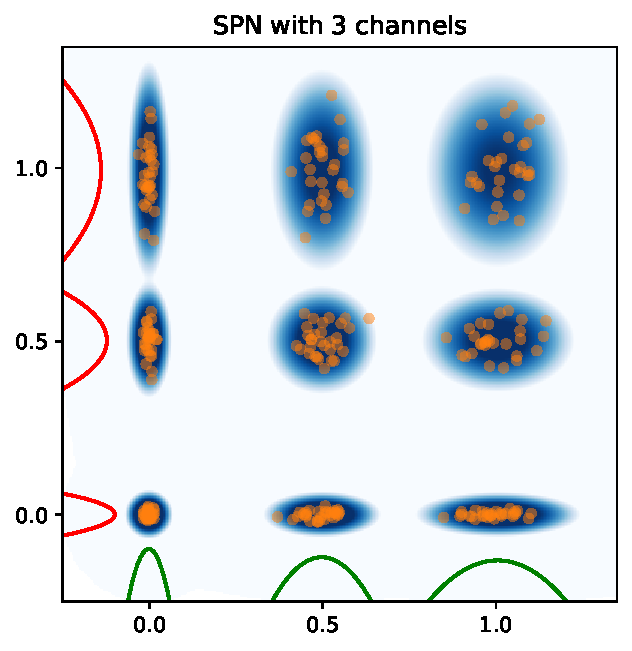
\includegraphics[width=0.46\textwidth]{Pictures/SPN_illustration1.pdf} }%
    \qquad
   {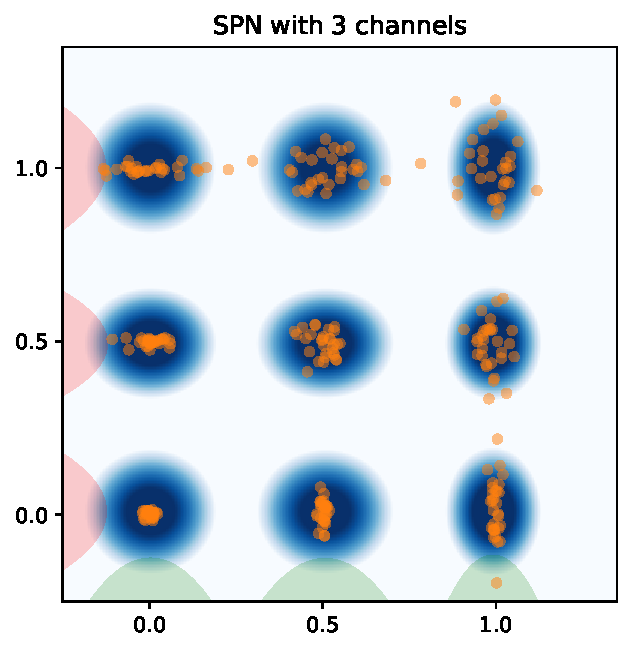
\includegraphics[width=0.46\textwidth]{Pictures/SPN_illustration2.pdf} }%
    \caption{SPN}%
    \label{SPN_fig}%
\end{figure}

\begin{figure}[htbp]
    \centering
    \begin{tikzpicture}

  % Define nodes

   % Define nodes
   \node[latent] (x4) {${x}_4$};
   \node[latent, left=of x4] (x3) {${x}_3$};
   \node[latent, left=of x3] (x2) {${x}_2$};
    \node[latent, left=of x2] (x1) {${x}_1$};
    \node[latent, left=of x1] (x0) {${x}_{0}$};
    
    \node[latent, below=of x4] (x4_hat){$\hat{{x}}_4$};
    \node[obs, below=of x3] (x3_hat){$\hat{{x}}_3$};
    \node[latent, below=of x2] (x2_hat){$\hat{{x}}_2$};
    \node[latent, below=of x1] (x1_hat){$\hat{{x}}_1$};
    \node[obs, below=of x0] (x0_hat){$\hat{{x}}_0$};
    
    \node[const, below= of x2_hat] (sigma-eps) {$\sigma_\epsilon$};
    \node[const, above= of x2] (sigma) {$\sigma$};

%   % Connect the nodes
%    \edge {I-0} {wifi-strength};
    \edge {x1} {x1_hat} ; %
    \edge {x0} {x0_hat} ;
    \edge {x2} {x2_hat} ; %
    \edge {x3} {x3_hat} ;
    \edge {x4} {x4_hat} ; %
    % \edge {a} {sensor-data} ; %

  \edge {x0} {x1} ; %
  \edge {x1} {x2} ; %
  \edge {x2} {x3} ; %
  \edge {x3} {x4} ; %
  
  \edge {sigma} {x1} ; %
  \edge {sigma} {x0}
    \edge {sigma} {x2} ; %
  \edge {sigma} {x3}
    \edge {sigma} {x4} ; %

  \edge {sigma-eps} {x1_hat} ; %
  \edge {sigma-eps} {x0_hat}
   \edge {sigma-eps} {x2_hat} ; %
  \edge {sigma-eps} {x3_hat}
   \edge {sigma-eps} {x4_hat} ; %
%    \plate{} {(wifi-location)(wifi-strength)(wifi-sensor)} {$K$}
%    \plate{} {(x)(x_)(wifi-sensor)(x_hat)} {$T$}
%    \plate{} {(x1)(x0)(x1_hat)} {$T$}    

%   % Plates
%   \plate {yx} {(x)(y)} {$N$} ;
%   \plate {} {(w)(y)(yx.north west)(yx.south west)} {$M$} ;
\end{tikzpicture}
    \caption{Model including wifi information}
    \label{fig:wifi2}
\end{figure}

\begin{figure}[H]
    \centering
    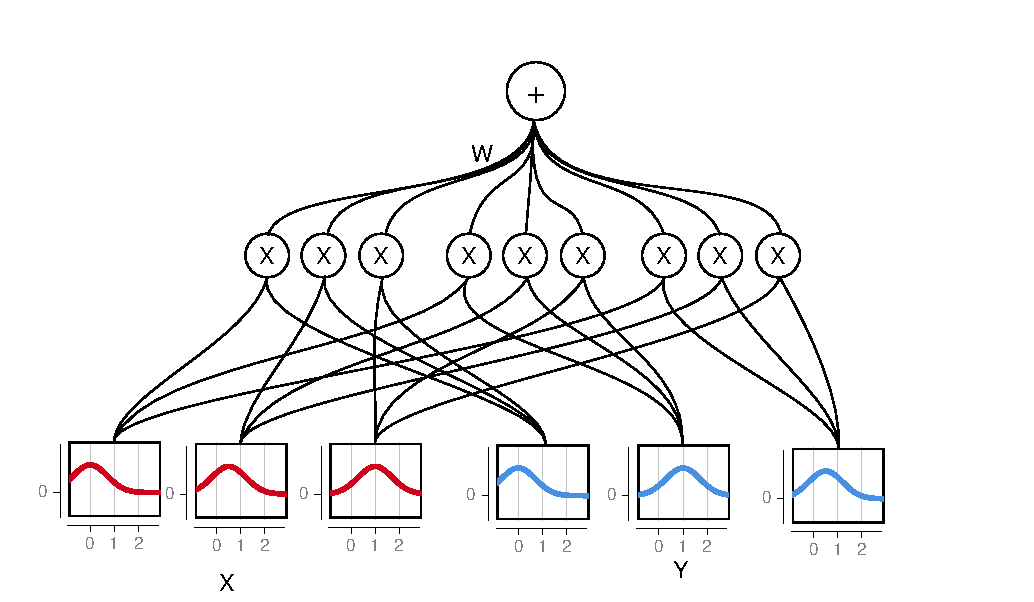
\includegraphics[width=\textwidth]{Figures/SPN_graph2.pdf}
\end{figure}
\cleardoublepage

\chapter{Inference: Prediction and learning}
Inference is the process of computing answers to queries about a probabilistic model after observing data. 
In Bayesian regression, the
query is the predictive distribution, $p(y|x,\mathcal{D})$, as we are interested in the distribution of $y$ given $x$ 
and already observed data, $\mathcal{D}$. 
This often indirectly create the posterior query, $p(\theta|\mathcal{D})$, the probability of model parameters $\theta$ given data
$\mathcal{D}$. Lastly it is also inference, when we train 
a Gaussian mixture model or SPN using the expectation-maximization algorithm (EM), since we are iteratively answering the query
$E_{p(z|\theta^{(k)})}[z|\theta]$.

\section{Exact and approximate inference}
We distinguish between two different ways of inference, exact and approximate inference.
It is \textit{exact inference} when a probabilistic query is calculated exact. It is possible to calculate exact inference on 
the predictive distribution for the Gaussian mixture model, Sum product network, and Gaussian processes. Models which allow 
for exact inference have a powerful advantage over the models with approximate inference since we can guarantee
 the answers to the queries are
correct, however, they are usually also less expressive. It is possible to
make exact inference of SPN, Gaussian Process, and Gaussian Mixture Regression. 
% \begin{itemize}
%     \item SPN
%     \item Gaussian Process
%     \item Gaussian Mixture Regression
% \end{itemize}

When it is not possible to answer a probabilistic query exact, we can approximate the
answer using \textit{approximate inference}. When dealing with complicated and expressive statistical models, exact inference is often
intractable and we need to use approximate inference. Approximate inference 
is a broad category of methods, which includes 
variational inference, Laplace approximation, and Markov chain Monte Carlo (MCMC).
The two Bayesian Neural networks we deal with in this project Bohamiann and Numpyro BNN are
similar regression models, but are infered using two different versions of the MCMC 
method, Hamiltonian Monte Carlo. As it will be revealed later (see result section) 
approximate inference might indeed be flawed and inexact. 
%When dealing with complicated and expressive statistical models, exact inference is often
%intractable and we need to use approximate inference, which might indeed be flawed and 
%inexact. 
% \begin{itemize}
%     \item Bohamiann (Adaptive stochastic MCMC)
%     \item Numpyro Bayesian Neural Network (NUTS)
% \end{itemize}

\begin{table}[H]
    \centering
    \begin{tabular}{l|l|l}
    %\rowcolor[HTML]{C0C0C0} 
    \textbf{Model} & \textbf{Predictive inference} &   \textbf{Learning} \\ \hline
    GP          & Exact $O(n^3)$  & Emperical Bayes\\
    SPN             & Exact $O(E)$ &  EM $O(E)$\\
    Gaussian Mixture Regression & Exact $O(K)$ & EM  \\
    Bohamiann                             & Adaptive stochatic HMC & \\
    Numpyro BNN                           & No U-Turn Sampler & 
    \end{tabular}
    \caption{Overview of inference methods applied on the statistical models 
            used in this project. $E$ is the number of edges in the SPN. $n$ is the number of datapoints. 
            $K \leq n$ is the number of mixture comonents. We will soon learn that for an
            SPN the number of mixture compenets is exponential larger than number of edges
            i.e. $E << K$. In theory MCMC methods samples 
            from true the posterior distribution, and do not need any fitting/learning. 
            }
\end{table}

\section{SPN}
Sum-product networks are generative models, i.e. statistical models of the joint distribution $p(x,y)$. 
We need, however, a disciminative model for regression, i.e. 
a model of the conditional distribution $p(y|x)$. 
SPNs allow for exact inference of the joint distribution 
and any marginalized distribution. These combined queries is sufficient for the
exact predictive posterior. 

\subsection{SPN - prediction}
Prior to the inference of the predictive distribution, we assume that the SPN, S, is trained, i.e.
trained leaf distributions $p_j(\cdot)$ for all leaf nodes, 
$j \in \mathcal{L}eaf(S):=\{j \in \mathcal{V}(S) |pa(j) = \text{Ø}\}$ and
weights $w_{i,j}$ for the connections between every sum nodes
$i \in \mathcal{S}$ and its children, $j \in ch(i)$.  
%The indexes of the nodes, are ordered such that leafs are first, and parents of leafs are next and then the grandparents and so on.

The joint and the marginal distribution are evaluated in the following recursive way
\begin{algorithm}
    \caption*{Calculation of $p(x,y)$}\label{SPN_1}
    \begin{algorithmic}
    \State \textbf{Input:} Fully trained SPN, with leaf distributions $p_i(\cdot)$ for $i\in \mathcal{L}eaf(S)$ and weigts 
    $w_{i,j}$ for $(i,j) \in \{(i,j)|i \in \mathcal{S}um(S), j \in ch(i)\}$ 
    \Function{\text{Eval}}{node i}
    \If{$i \in \mathcal{L}eaf(S)$}
        \State  $\textbf{return: } p_i(x,y)$ \Comment{evaluate leaf distributions at point $(x,y)$}
    \EndIf
    %\For{$i \in I_{o}$}
    \If{$i\in \mathcal{S}um(S)$}
        \State $\textbf{return: } \sum_{j\in ch(i)} w_{i,j} \text{Eval}(j)$
    \EndIf
    \If{$i\in \mathcal{P}rod(S)$}
        \State $\textbf{return: } \prod_{j \in ch(i)} \text{Eval}(j)$
    \EndIf
    \EndFunction
    \State $p(x) =  \text{Eval(root)}$
    \end{algorithmic}
\end{algorithm}

\begin{algorithm}[H]
    \caption*{Calculation of $p(x)$}\label{SPN}
    \begin{algorithmic}
    \State \textbf{Input:} Fully trained SPN, with leaf distributions $p_i(\cdot)$ for all leaves $i$ and weigts $w_{\cdot,\cdot}$ 
    \Function{\text{Eval}}{node i}
    \If{$i \in \mathcal{L}eaf(S)$} %\Comment{leaf node}
        \If{node handle x}
            \State  $\textbf{return: } p_i(x,y)$ \Comment{evaluate leaf distributions at point $(x,y)$}
        \Else 
            \State  $\textbf{return: } 1$ \Comment{set node equal 1 at point $(x,y)$}
        \EndIf
    \EndIf
    \If{$i\in \mathcal{S}um(S)$}
        \State $\textbf{return: } \sum_{j\in ch(i)} w_{i,j} \text{Eval}(j)$
    \EndIf
    \If{$i\in \mathcal{P}rod(S)$}
        \State $\textbf{return: } \prod_{j \in ch(i)} \text{Eval}(j)$
    \EndIf
    \EndFunction
    \State $p(x) =  \text{Eval(root)}$
    \end{algorithmic}
\end{algorithm}

So after doing two slightly different forward passes through the SPN, 
$p(x)$ and $p(x,y)$, using Bayes rule,
we can combined the two queries into the conditional distribution: 
$$p(y|x) = \frac{p(x,y)}{p(x)}$$
The predictive distribution is found with a cost of just $O(E+E+1) = O(E)$, where E is number
of edges/connections in the SPN. 

\subsection{SPN - learning}
It is not enouth to do predictive inference on a SPN, we also need to fit it on
the data. It is possible interpret sum-product network as a large mixture model 
and therefore use expectation-maximization to train the model. 
We will introduce that idea now. The Paper \cite{SPN_EM}... %["Learning Arbitrary Sum-Product Network Leaves
%with Expectation-Maximization"] 
defines SPN as a mixture of all sub-networks of an SPN.

%from [@desana]:
\begin{definition} 
    A sub-network $\bar S_z$ of $S$ is an SPN, which includes the root $S$ and then includes nodes
    according to the following recursive scheme: 
\end{definition}
\begin{algorithm}[H]
    \caption*{Collection of sub-network $S_z$ of $S$}\label{SPN3}
    \begin{algorithmic}
    %\State \textbf{Global:}  $S_z$ 
    \Function{Process}{node i, $S_z$}
    \If{$i \in \mathcal{L}eaf(S)$}
        \State  $\textbf{return: }$ 
    \EndIf
    %\For{$i \in I_{o}$}
    \If{$i\in \mathcal{S}um(S)$}
       %\State $S_z =S_z \cup \{j \in ch(i)\}$ \Comment{include one child of node $i$}
        \State $S_z =S_z.add(j \in ch(i))$ \Comment{include one child of node $i$}
        \State $\textbf{return: } \text{Process}(j, S_z)$
    \EndIf
    \If{$i\in \mathcal{P}rod(S)$}
        \State $S_z =S_z \cup \{j | j \in ch(i)\}$ \Comment{include all childen of node $i$}
        \For{$j \in ch(i)$}
            \State $\textbf{return: } \text{Process}(j,S_z)$
        \EndFor
    \EndIf
    \State $\textbf{return: } S_z$
    \EndFunction
    \State $S_z =  \text{Process(root,Ø)}$
    \end{algorithmic}
\end{algorithm}
So we see that at each sum node the number of different sub-networks multiplies with the number of children for that
sum node. And thereby, the total number of sub-networks is
 $$Z = \prod_{i\in \mathcal{S}um(S)}|ch(i)|$$ 
 i.e. an exponential large amount of sub-networks. This is the amount of
 mixture components implicitly defined in an SPN. 
 Denote the set of edges in the sub-network $\mathcal{E}(S_z)$.
Now the we define a mixture coeficient, $\lambda_z$ and component for each $S_z$ as 
$$\lambda_z := \prod_{(i,j)\in \mathcal{E}(S_z)} w_{i,j}, \hspace{1cm}
p_z(x,y|\theta) := \prod_{i \in \mathcal{L}(S_z)} p_i(x,y)$$
where $p_i(x,y)$ is the leaf distribution at leaf node $i$ paramitised with $\theta$. 
It can now be proven that the SPN can be interpreted as the following mixture model, 
$$p(x,y|w,\theta) = \sum_{z=1}^Z \lambda_z(w)p_z(x,y|\theta)$$
i.e. by the weighted sum of all $Z$ sub-networks. For convinience
we define each sum component as $p(z,x,y|w,\theta) := \lambda_z(w)p_z(x,y|\theta)$.
Evaluation of $p(x,y|w,\theta)$ will never be done as the sum over $Z$ components, 
instead there is a proposition. 

\begin{proposition}
    Consider a SPN, S, a sum node $q \in \mathcal{S}um(S)$ and a child $i \in ch(q)$,
    then the following relation holds, 
    $$\sum_{z:(q,i)\in \mathcal{E}(S_z)} \lambda_z(w) p_z(x,y|\theta) = w_{i,q}
    \frac{\partial S}{\partial v(q)} v(i)$$
\end{proposition}

\newpage
\section{Expectation-maximization for mixture models}
Mixture models can be seen as probibalistic graphical models, <fig> there one mixture component is
picked according to the realization of a catagorical variable $\textbf{Z}$ with parameters according
the the mixture weights, i.e we can reformelate, 
\begin{align*}
    p(x) &= \sum_{k=1}^K w_k p_k(x)\\
   \iff \hspace*{1cm} p(x) &= p_z(x), \hspace*{0.5cm} z \sim Cat(w_i, \dots, w_K).
\end{align*}
In fact $p_z(x)$ is a conditial distribution, $p(x|z)$, and combined with the distribution
of $Z$ we can define the joint 
$$p(x,z):=p_z(x)p(z)$$
The the case of a statistical model, data $\mathcal{D}$ is fitted by the mixture model 
by tuning the model parameters $\theta = \{w, \text{paramers for} p_i\}$. Then the joint
distribtuion $p(\mathcal{D},z| \theta)$ is refered as the \textit{complete-data} likehood in the EM algorithm. 
$$p(\mathcal{D},z|\theta):=p(\mathcal{D}|z,\theta)p(z|\theta)$$ 
When fitting model parameters we essentially want to find the parameters, that maximize the probability of
the parameters given the data, $p(\theta|\mathcal{D})$. Assuming an
unimformative/flat prior $p(\theta)$, 
\begin{align*}
p(\theta|\mathcal{D})&= \frac{p(\mathcal{D}|\theta)p(\theta)}{p(\mathcal{D})}\\
\Rightarrow  \arg\max_{\theta} p(\theta|\mathcal{D}) &= \arg\max_{\theta} p(\mathcal{D}|\theta)
\end{align*}
we arrive at the maximum likelihood estimate (MLE). The task of finding the MLE is conviniently
done using EM algorithm, since we can look at the likehood as the marginalized
\textit{complete-data} likehood, 
$$p(\mathcal{D}|\theta) = \sum_z p(\mathcal{D}, z|\theta)$$

%(Note that this statement true accoring to Theorem 2.1. in \cite{gupta2011theory}). 

\begin{testexample2}[Expectation-maximization EM <based on Bishops book>]
    Expectation maximization is a convinient method for finding ML (or MAP) estimate of a 
    latent variable model. We consider a probibalistic model paramitised with $\theta$, 
    $$p(\textbf{X}, \textbf{Z}|\theta)$$ where we denote all latent variables \textbf{Z}, and
    observed variables \textbf{X}. Our goal is to find the maximum of the likehood, 
    $$p(\textbf{X}|\theta) = \int p(\textbf{X}, \textbf{Z}| \theta) \mu(d\textbf{Z})$$
    maximizating the likehood itself $p(\textbf{X}|\theta)$ is assumed dificult 
    but maximizating of the \textit{complete-data} likehood $p(\textbf{X}, \textbf{Z}|\theta)$
    is much easier. The algorithm iterates over two steps: The expecation (E) step and the maximization (M) step, 
    defined in the following way for iteration $t$, 
    
    \textbf{E-step}

    Define the functional $Q(\theta,\theta^{(t)})$, to be the expected value of the complete-data 
    log likehood (log likehood function of $\theta$), with respect to the only random quantaty $\textbf{Z}$,
    which is assumed to follow a distribtuion with the density $p(\textbf{Z}|\textbf{X}, \theta^{(t)})$,
    i.e. the conditional distribution of \textbf{Z} given \textbf{X} and the current parameter point estimate
    $\theta^{(t)}$: 
    $$Q(\theta,\theta^{(t)}) := E_{p(\textbf{Z}|\textbf{X}, \theta^{(t)})}[\log p(\textbf{X}, \textbf{Z}|\theta)]$$

    \textbf{M-step}

    After the E-step we find the point estimate $\theta^{(t+1)}$ which maximizes $Q(\cdot|\theta^{(t)})$, i.e.
    $$\theta^{(t+1)} = \arg\max_{\theta} Q(\theta|\theta^{(t)})$$

    \begin{algorithm}[H]
        \caption*{(local) maximization of $p(\mathcal{D}|\theta)$}\label{EM}
        \begin{algorithmic}
        \State \textbf{Input:} dataset $\mathcal{D}$, joint model $p(\mathcal{D}, \textbf{Z}|\theta)$
        \While{Not converged}
            \State $Q(\cdot, \theta^{(t)}) \gets E_{p(\textbf{Z}|\mathcal{D}, \theta^{(t)})}[\log p(\mathcal{D}, \textbf{Z}|\theta)]$ \Comment{E-step}
            \State $\theta^{(t+1)} \gets \arg\max_{\theta} Q(\theta|\theta^{(t)})$ \Comment{M-step}
        \EndWhile
        \State $\textbf{return: } \theta^{(end)}$
    \end{algorithmic}
    \end{algorithm}

    \textbf{Proof of correctness} 
    
    We will now give a short proof that maximizing $Q(\cdot|\theta^{(t)})$ maximizes the likelihood
    $p(\textbf{X}|\theta)$, where we assume that $\textbf{Z}$ is a random vector with a discrete
    distribution. This allow us to use Gibbs inequality: 
    $$\sum_z p_1(z) \log p_1(z) \geq \sum_z p_1(z) \log p_2(z)$$ where $p_1(\cdot)$ and $p_2(\cdot)$
    are densities belonging to two discrete distributions of $Z$, equality if $p_1(\cdot) =
    p_2(\cdot)$. From now on we will alter the subscript on the expecations, just have in mind that
    $$E_{\theta^{(t)}}[g(Z)]:=E_{p(\textbf{Z}|\textbf{X}, \theta^{(t)})}[g(Z)] = \sum_z g(z)
    p(\textbf{z}|\textbf{X}, \theta^{(t)})$$ 
    Now to the proof: From bayes rule $p(\textbf{X}|\theta) =
    \frac{p(\textbf{X}, \textbf{Z})}{p(\textbf{X})}$ we can write
    $$\log p(\textbf{X}|\theta) = \log p(\textbf{X}, \textbf{Z}) - \log p(\textbf{Z}|\textbf{X},\theta)$$
    Now, taking the expecation of the above w.r.t. $p(\textbf{Z}|\textbf{X}, \theta^{(t)})$,
    yields,
    \begin{align*}
        \log p(\textbf{X}|\theta)  &= E_{\theta^{(t)}}[\log p(\textbf{X}, \textbf{Z}|\theta)]
        -  E_{\theta^{(t)}}[\log p(\textbf{Z}|\textbf{X},\theta)]\\
        &= Q(\theta,\theta^{(t)})+ E_{\theta^{(t)}}[\log p(\textbf{Z}|\textbf{X},\theta)]
    \end{align*} 
    Since the above equation holds for any $\theta$, it also holds for $\theta^{(t)}$
    now we have, 
    $$\log p(\textbf{X}|\theta^{(t)}) = Q(\theta^{(t)},\theta^{(t)})+ E_{\theta^{(t)}}[\log
    p(\textbf{Z}|\textbf{X},\theta^{(t)})]$$ 
    Subtracting the two equations, we get,  
    $$\log p(\textbf{X}|\theta) - \log p(\textbf{X}|\theta^{(t)}) = Q(\theta,\theta^{(t)})
    -Q(\theta^{(t)},\theta^{(t)})+ E_{\theta^{(t)}}[\log p(\textbf{Z}|\textbf{X},\theta)]-
    E_{\theta^{(t)}}[\log p(\textbf{Z}|\textbf{X},\theta^{(t)})]$$ From Gibb's inequality we have
    that $E_{\theta^{(t)}}[\log p(\textbf{Z}|\textbf{X},\theta^{(t)})]\leq E_{\theta^{(t)}}[\log
    p(\textbf{Z}|\textbf{X},\theta)]$ where equality only holds for $\theta^{(t)} = \theta$, giving
    \begin{align*}
        \log p(\textbf{X}|\theta) - \log p(\textbf{X}|\theta^{(t)}) \geq 
    Q(\theta,\theta^{(t)})
    -Q(\theta^{(t)},\theta^{(t)})
    \end{align*}
    so optimizing $Q(\theta,\theta^{(t)})$ will optimize
    $\log p(\textbf{X}|\theta) $ as least as much.
\end{testexample2}


then we can marginalise over
    $z$ in order to recover $p(x)$, 
    $$p(\textbf{x}|\pi) = \sum_{z=1}^Z p(z,\textbf{x}|\pi) $$
    assuming iid data, then the complete likehood can be decompose as the product 
    $$ p(z,\textbf{x}|\pi) = \prod_{i=1}^n p(z,\textbf{x}_i|\pi)$$
    We wil for convinience transform the likelihood using a log transform, 
    as it will not influence the maximum. 
    $$\log p(\textbf{x}|\pi) = \sum_{z=1}^Z \sum_{i=1}^n \log p(z,\textbf{x}_i|\pi)$$

<EM for SPN >
<EM for GMM >

% and a normal evaluation of $p(x,y|w_{old}, \theta_{old})$
% combined in Bayes rule we obtain
% $$p(z|x,y,w_{old},\theta_{old}) = \frac{p(z,x,y|w_{old},\theta_{old})}{p(x,y|w_{old}, \theta_{old})} =
%  \frac{\lambda_z(w_{old})p_z(x,y|\theta_{old})}{p(x,y|w_{old}, \theta_{old})} $$

% and we have the expecation for the EM-algorithm, 
% $$Q(\pi, \pi_{old}) = \sum_{n=1}^N \sum_{z=1}^Z p(z|xy_n, \pi_{old}) \ln p(z,xy_n|\pi)$$

\begin{tcolorbox}[
    sharp corners,
    boxrule=0mm,
    enhanced,
    borderline west={2pt}{0pt}{red},
    colframe=drGray,
    colback=drGray,
    coltitle=black,
]
{\large \textbf{Her er en titel}}
\begin{itemize}
    \item Lorem ipsum dolor sit amet, consectetur adipiscing elit. Proin euismod finibus enim vel tincidunt. Aliquam a placerat risus. Donec lobortis consequat massa et rhoncus. Cras a quam nec ante porta consequat at in nulla. Praesent sagittis, tortor id iaculis pharetra, dui eros gravida 

\item Cras euismod mauris ut magna porta egestas. Ut non nisl leo. In hac habitasse platea dictumst. Pellentesque sed diam hendrerit tellus sagittis bibendum. Donec lorem augue, aliquet 

 \item In at interdum lacus. Ut purus arcu, consequat a leo at, viverra tincidunt eros. Sed non mi fringilla, ornare velit eget, feugiat tortor. Donec blandit orci at dapibus vehicula. Pellentesque non cursus tellus. Ut et molestie quam. Sed convallis laoreet odio at dignissim. Maecenas condimentum felis eu laoreet pretium. Fusce lacinia ligula purus, non
\end{itemize}
\end{tcolorbox}

\section{Gaussian Mixture Regression}
The Gaussian mixture is a generative model of the joint probability of $x$ and $y$ given as, 
$$p(x,y)= \sum_{k=1}^K \pi^{(k)} \mathcal{N}(x,y|\mu^{(k)},\Sigma^{(k)}), 
\hspace{1cm} \mu=\begin{bmatrix}
    \mu_x \\ \mu_y
\end{bmatrix},\hspace{0.1cm} \Sigma = \begin{bmatrix}
    \Sigma_{xx} & \Sigma_{xy}\\ \Sigma_{yx}& \Sigma_{yy}
\end{bmatrix}$$
This is trained using the EM algorithm. We will now show how the conditial is
calculated exact. 
\subsection{GMR - prediction}
We need the conditional distribution of the Gaussian mixture
in order to get the predictive distribution. We will now formulate
the conditial distribution in terms of conditional and marginals of
the individual mixture components. First of all the marginal distribution $p(x)$ 
of the mixture is given as, \todo{How??!}
$$p(x) = \sum_{k=1}^K \mathcal{N}(x|\mu_{x}^{(k)},\Sigma_{xx}^{(k)})$$ 
next the joint distribution can be decomposed with the probability chain rule,
\begin{align*}
    p(x,y) &= p(x)p(y|x)\\
    \implies \hspace{1cm} \mathcal{N}(x,y|\mu,\Sigma) &= 
    \mathcal{N}(x|\mu_{x},\Sigma_{xx}) \mathcal{N}(y|\mu_{y|x},\Sigma_{y|x})
\end{align*} 
And we can formulate the conditial in terms of individual multivariate Gaussians, 

\begin{align}
    p(y|x) &= \frac{p(y,x)}{p(x)}\\
    &= \sum_{k=1}^K \frac{\pi^{(k)}}{p(x)} \mathcal{N}(x,y|\mu^{(k)},\Sigma^{(k)})\\
    &=  \sum_{k=1}^K \frac{\pi^{(k)} \mathcal{N}(x|\mu_{x}^{(k)},\Sigma_{xx}^{(k)})}{p(x)}\mathcal{N}(y|\mu_{y|x}^{(k)},\Sigma_{y|x}^{(k)})\\
    &=  \sum_{k=1}^K \pi_{y|x}^{(k)} p(y|x,\mu_{y|x}^{(k)},\Sigma_{y|x}^{(k)})
\end{align}

where $\pi_{y|x}^{(k)} := \frac{\pi^{(k)} \mathcal{N}(x|\mu_{x}^{(k)},\Sigma_{xx}^{(k)})}
{\sum_{i=1}^K \mathcal{N}(x|\mu_{x}^{(i)},\Sigma_{xx}^{(i)})}$. So we see that 
the conditonal of a Gaussian mixture model is again a Gaussian mixture model.


\begin{testexample2}[Conditional og multivariate Gaussian]
    The conditional distribution is defined as <ref bishop>
    $$p(y|x,\mu, \Sigma) = \mathcal{N}(y|\mu_{y|x},\Sigma_{y|x} )\hspace{1cm} \mu=\begin{bmatrix}
        \mu_x \\ \mu_y
    \end{bmatrix},\hspace{0.1cm} \Sigma = \begin{bmatrix}
        \Sigma_{xx} & \Sigma_{xy}\\ \Sigma_{yx}& \Sigma_{yy}
    \end{bmatrix}$$ 
    where 
    \begin{align}
        \mu_{y|x} &= \mu_y+\Sigma_{yx}\Sigma_{xx}^{-1}(x-\mu_x)\\
        \Sigma_{y|x} &= \Sigma_{yy}-\Sigma_{yx}\Sigma_{xx}^{-1}\Sigma_{xy} 
    \end{align}
    
\end{testexample2}


\subsection{GMR - Leaning}

EM-algorithm, classic example. 

\section{Gaussian Process Regression}
We now show how the preditive distribution is calculated exact for
Gaussian Processes, i.e. 
\begin{equation}\label{GP_predictive}
    p(y|x,\mathcal{D}) = \int \mathcal{N}(y|f(x), \sigma^2) p(f(x)|\mathcal{D})df(x)
\end{equation}
we will soon see that $p(f(x)|\mathcal{D}) = \mathcal{N}(f(x)| .., ...)$ and
and thereby that we have a marginal Gaussian distribution for $f(x)$ and a 
conditional Gaussian distribution of $y$ given $f(x)$, giving us the marginalized
distribtuion, $p(y|x,\mathcal{D})$, using formulars \eqref{marginal_distribution}. 

\begin{testexample2}[Trick with normal distributions [from Bishops book?]]
    Given a marginal Gaussian distribution of $x$ and a conditional Gaussian distribution
    of $y$ given $x$ of the form, 
    \begin{align*}
        p(x) &= \mathcal{N}(x|\mu, \Lambda^{-1})\\
        p(y|x) &= \mathcal{N}(x|Ax+b, L^{-1})
    \end{align*}
    then the marginal distribution of $y$ and the conditional distribution of $x$ given $y$
    have the form, 
    \begin{align}
        p(y) &= \mathcal{N}(y|A\mu+b,L^{-1}+A \Lambda^{-1}A^T) \label{marginal_distribution}\\
        p(x|y) &= \mathcal{N}(x|\Gamma \mu+\Gamma [A^TL(y-b)],\Gamma )\\
        \Gamma &:= (\Lambda +A^TLA)^{-1}
    \end{align}
\end{testexample2}

\subsection*{Posterior function}
Recall we assume $\textbf{f} = (f(\textbf{x}_1), \dots, f(\textbf{x}_n))$ is the parameters in 
our model, therefore we call $p(\textbf{f}|\mathcal{D})$ the posterior distribution. However, 
what is of real interest is the function values on unobserved locations, thereby we 
extend $\textbf{f}$ to be a function, i.e. an infinitely dimentional vector. We call this 
quantaty \textit{the posterior function} 
\begin{equation}\label{posterior_function}
    p(f(\cdot)|\mathcal{D})= \int p(f(\cdot)|\textbf{x}, \textbf{f})p(\textbf{f}|\mathcal{D})d\textbf{f}.
\end{equation}
% The connection between the two posteriors is given here:
% $$p(f(\cdot)|\mathcal{D}) = \int p(f(\cdot)|\textbf{x}, \textbf{f})p(\textbf{f}|\mathcal{D})d\textbf{f}$$
Prior we assume that the function takes values accoring to
$$p(\textbf{f}|\textbf{x}) = \mathcal{N}(\textbf{f}|\textbf{0}, c(\textbf{x}, \textbf{x}))$$
where the covariance is defined at kernel evaluation for each pair of $\textbf{x}$,
where $c(\cdot, \cdot)$ is a covariance function, chosen to be the Matérn covariance function,

  $$c(\textbf{x}, \textbf{x}) = \begin{bmatrix}
    c(x_1,x_1) & \dots & c(x_1,x_n)\\
    \vdots& \ddots\\
    c(x_n,x_1) & \dots & c(x_n,x_n)
\end{bmatrix}\hspace{1cm} c(x, y) := Matern(x,y)...$$ 

We now calculate the first term in the integral \eqref{posterior_function}, 
$p(f(\cdot)|\textbf{x}, \textbf{f})$ using that we have the joint prior 
distribution, 
\begin{align}
    p(f(\cdot),\textbf{f}|\textbf{x}) = \mathcal{N}\left(\begin{bmatrix}
        f(\cdot)\\ \textbf{f}
    \end{bmatrix} \middle| \begin{bmatrix}
        0\\ \textbf{0}
    \end{bmatrix}, \begin{bmatrix}
        c(\cdot, \cdot) & c(\cdot,\textbf{x})\\
        c(\textbf{x}, \cdot) & c(\textbf{x}, \textbf{x})
    \end{bmatrix} \right)
\end{align}

And the conditonal of a joint Gaussian is given using <ref> 
$$p(f(\cdot)|\textbf{x}, \textbf{f}) = \mathcal{N}(f(\cdot)|c(\cdot, \cdot)^{-1}c(\cdot, \textbf{x})\textbf{f}, c(\cdot, \cdot)^{-1})$$

Next we calculate the last term in the integral \eqref{posterior_function}, 
$p(\textbf{f}|\mathcal{D})$, i.e. the posterior distribution. Assuming iid data, 
i.e. $p(y_1,\dots, y_n|x_1,\dots, x_n, \textbf{f}) = \prod_{i=1}^n p(y_i|x_i,\textbf{f}_i)$
and that the likelihood is Gaussian with mean $\textbf{f}$ and variance $\sigma^2 I_n$. 

\begin{align*}
    p(\textbf{f}|\mathcal{D}) &\propto p(\textbf{f}|x)\prod_{i=1}^n p(y_i|x_i,\textbf{f}_i)\\
    &= \mathcal{N}(\textbf{f}|\textbf{0},c(\textbf{x}, \textbf{x})) \prod_{i=1}^n \mathcal{N}(y|\textbf{f}_i,\sigma^2)\\
    &= \mathcal{N}(\textbf{f}|\textbf{0}, c(\textbf{x}, \textbf{x})) \mathcal{N}(\textbf{y}|\textbf{f},\sigma^2 I_n)
\end{align*}
now from <ref> we have that the posterior is the following Gaussian: 
\begin{equation*}
    p(\textbf{f}|\mathcal{D}) = \mathcal{N}(\textbf{f}|M^{-1} \sigma^{-2}\textbf{y}, M^{-1}) \hspace{0.5cm}M := c(\textbf{x}, \textbf{x})^{-1}+\sigma^{-2} I_n
\end{equation*}
Now we found that both term in the integral \eqref{posterior_function}, and they
are related such that it is possible to use \eqref{marginal_distribution} for arriving 
at (we define $A :=  c(\cdot, \cdot)^{-1} c(\cdot, \textbf{x})$), 
$$p(f(\cdot)|\mathcal{D}) = \mathcal{N}(f(\cdot)|AM^{-1}\sigma^{-2}\textbf{y}, c(\cdot, \cdot)^{-1}+
AM^{-1}A^T)$$

Finally we found that both terms in the integral \eqref{GP_predictive} also is related
in a simlar way, and we use \eqref{marginal_distribution}, again to arrive at the predictive
distribtuion, 
$$p(y_*|x_*,\mathcal{D}) = \mathcal{N}(y_*|AM^{-1}\sigma^{-2}\textbf{y}, c(x_*, x_*)^{-1}+
AM^{-1}A^T+\sigma^2)$$

\todo{Some questions about a naive approach..!}

\subsection*{Learning - Emperical bayes inference}

Anther inference which is done is then optimizing the hyper parameters using emperical bayes i.e.
the variance and length scale for the kernel. Here we optimize the marginalized likelihood function
$$p(y_1, \dots, y_n|x_1, \dots, x_n, \theta) = -\frac{1}{2}[(y-\mu)^T (\Sigma+N)^{-1}(y-\mu)+ \log |\Sigma+N|+n \log 2\pi]$$
<and how to get to there?>

\todo{Model assessment becomes trivial in light of the model posterior if we
simply establish preferences over models according to their posterior
probability. When using the uniform model prior (4.6)
 the model posterior is proportional to the marginal likelihood alone,
which can be then used directly for model assessment. ??! Forstår ikke}

\section{Deep Network Global Optimization - ?} ??
Kernel regression :-))
Should I not work on this?

\section{Bayesian Neural Networks}
Bohamiann and numpyro-BNN are examples of probabilistic models with intractable inference. The predictive density is given as, 
\begin{align*}
    p(y_*|x_*,\mathcal{D}) &= \int p(y_*|x, \theta)p(\theta|\mathcal{D})d\theta\\
    &\approx \frac{1}{K} \sum_{k=1}^K p(y_*|x, \theta^{(k)})
\end{align*}
where the first integral is intractable as $\theta$ can live in a highly dimensional space, second the approximation sign
is true, since we can aproximate the integral with monte carlo sampling: $\theta^{(k)}$ are iid samples from the posterior 
distribution, $\theta^{(k)} \sim p(\theta|\mathcal{D})$. We can get samples from the posterior distriution

\begin{testexample2}[Monte Carlo approximation]
    Assuming we have a number of iid samples, $\theta^{(1)}, \dots, \theta^{(K)}$ drawn from the
    distribution $p(x)$, then the following appriximation 
    $$E[f(x)] \approx \frac{1}{K} \sum_{k=1}^K f(x^{(k)}) =: \Theta_{K}(f)$$
    holds accoring to the law of large numbers 
    in fact $$E[f(x)] = \lim_{K \rightarrow \infty} \Theta_{K}(f)$$
    and the central limit theorem, <OBS refere!>
    $$p(\hat \Theta) \approx \mathcal{N}(\hat \Theta |\mu_f, \frac{\sigma_f^2}{K})$$
    which ensures that the variance of the unbiased estimator of the expecation decreases
    with number of samples, $K$. Left is to sample the $iid$ samples from the distribution $p(x)$
\end{testexample2}
\subsection*{Posterior samples}
For both models 
the joint distribution $p(\mathcal{D},\theta)$ is available, but calulating the posterior distribution requires the
marginalized likehood, $p(\mathcal{D}) = \int_{\theta} p(\mathcal{D},\theta)$. This integral is often intractable
since the space of $\theta$ typically is abnomous - so not even nummerical appriximations of the intergral is tractable.
From Bayes rule, we have the equality, 
$$p(\theta|\mathcal{D}) = \frac{p(\mathcal{D},\theta)}{p(\mathcal{D})} \propto p(\mathcal{D},\theta),$$
where the propotional sign is true, since $p(\theta|\mathcal{D})$ is a function of $\theta$. 
Knowing the $p(\mathcal{D},\theta)$ joint distribution thereby allow for using Markov chain Monte Carlo
for sampling from the posterior distribution.  

\begin{testexample2}[Markov chain Monte Carlo]
    We can conviniently use MCMC for sampling from a probability density $p(x)$, with only the knowledge of a 
    propotional/unnormalised density $\hat p(x) \geq 0$ i.e
    $$\hat p(x) = c\cdot p(x) \hspace{1cm} c = \int \hat p(x) dx,$$
    where $\int \hat p(x) dx$ is a possible intractable integral. 
    An ergodic Markov chain/process is constructed, such that its stationary distribution is exactly $p(x)$, but only
    with the knowledge of $\hat p(x)$. 
\end{testexample2}

\begin{testexample}[Metropolis-Hasting (MH)]
    The most simple MCMC method is the Metropolis-Hasting algorithm. At iteration
    $n$ we have a sample $x_n$,
    \begin{enumerate}
        \item Propose $\hat x$ from a proposal density $q(x_n,\cdot)$
        \item Compute accptance probability $$\alpha(x_n,\hat x) = \min \left(1, \frac{p(\hat x)}{p(x_n)} \frac{q(\hat x, x_n)}{q(x_n,\hat x)}\right)$$
        \item Set the next sample $$x_{n+1} = \begin{cases}
            \hat x &\text{with probability } \alpha(x_n, \hat x)\\
             x_n &\text{with probability } 1-\alpha(x_n, \hat x)
        \end{cases}$$
    \end{enumerate}
    note that $\alpha(x_n,\hat x)$ requires $p(x)$, but since the algorithm only
    requires the fraction $\frac{p(\hat x)}{p(x_n)} = \frac{p(\hat x)\cdot c}{p(x_n)\cdot c} = \frac{\hat p(\hat x)}{\hat p(x_n)}$
    we only need $\hat p$. 
    
    \textbf{Proof:} Assuming discrete states, the transition probability between the states are given as, 
    $$p(x\rightarrow y) = \begin{cases}
        q(x,y)\alpha(x,y) & \text{if } x\neq y\\
        q(x,x) + \sum_{z\neq x} q(x,z)(1-\alpha(x,z)) & \text{if } x=y
    \end{cases}$$
    Now, let us look at the so-called \textit{detailed balance} relation, i.e. that if we are sampling from the
    stationary density we stay there at the next state. Assume $x\neq y$, 
    \begin{align*}
        p(x)p(x\rightarrow y) &= p(x)q(x,y)\alpha(x,y)\\
        &=p(x)q(x,y) \min \left(1, \frac{p(\hat x)}{p(x_n)} \frac{q(\hat x, x_n)}{q(x_n,\hat x)}\right)\\
        &= \min(p(x)q(x,y), p(y)q(y,x))
    \end{align*}
    Observing that the right hand side yields symmetric result in $x$ and $y$, therefore we obtain, 
    $$p(x)p(x\rightarrow y) = p(y)p(y\rightarrow x)$$
    and summing over $x$ on both sides yields,
    \begin{align}
        \sum_x p(x)p(x\rightarrow y) &= p(y) \sum_x p(y\rightarrow x)\\
        \implies \hspace{0.5cm} p(y) &= \sum_x p(x)p(x\rightarrow y)
    \end{align}
    similar conclusion will be obtained for $x = y$, all in all this reveals that $p(x)$ is in fact invariant for the chain
     $\{x_1, \dots , x_n\}$ and thereby that MH is a MCMC algorithm. 
\end{testexample}

% Markov assumption -> history doesn't matter
% Monte Carlo -> Random simulation
% best methods, use gradients. 

% Simulared skate board in a state park. Physic simulation. 
% Often the simulation moves back and fouth and end up in the 
% same point - this is called a U-turn. 

% find global curvature from just knowing the local curvature. 
% Simulation is moving more in the area with high prob. mass. 

% Gradients: Automated differentiation. 

% We want to evaluate integrals of the fom $$E[f(x)] = \int f(x)p(x)dx$$ where $x \in \mathbb{R}^n$ is a
% random vector under the distribution $p(x)$. we are interested in problems where the form of $f(x)$ or $p(x)$
% makes the integral intractalbe. 

% \begin{testexample}[Bayesian neural network]
%     Choosing $f := \mathcal{N}(y;NN_w(x), \sigma)$ and looking at $\theta := (w,\sigma)$ as the random quantaty
%     under the posterior distribution $p(\theta|\mathcal{D})$ we indeed have case of a intractalbe expectation
% \end{testexample}



% Transition density kernel (transtion matrix for finite discrete spaces) $p(x^{(k)}|x^{(k-1)})$



% c) the convergence rate is independent on the
% dimensionality, l. The latter property is in contrast to methods based on the deterministic numerical
% integration, which, in general, have a rate of convergence that slows down as the dimensionality
% increases.

HM with random walk transition is very simple and it comes with some serious disadvantages:
slow convergence speed, might stay in the same region for a long time and produces highly correlated sampels. 
We can do better by replacing the random walk with gradient-guided movements and intepretate the probability
landscape as a physical system.


\begin{testexample}[HMC]
The golden standard in MCMC is the Hamilton monte carlo, which exploits arguments from classical mechanics
around the Hamiltonian equations. This method leads to more efficient sampling as the Hamiltonian intepretation allows the system
to take regions with high probability mass into acound - this is optained using gradient
of the probability landscape.  $\frac{-\partial E(x)}{\partial x} $
 
We define PDF
$$p(x) = \frac{1}{Z_E}\exp(-E(x)),$$

where $E(x)$ is interpretted as the systems potential energy. Now, an latent vector $q$ is introduced in order
to represent the momentum of the system, which gives us the kinetic energy of the system. 

$$K(q) = \frac{1}{2}\sum_{i=1}^l q_i^2$$

Giving the Hamilton function and its coresponing distribution

$$H(x,q)= E(x)+K(q)$$

and 
\begin{align}
    p(x,q) &= \frac{1}{Z_H} \exp(-H(x,q))\\
    &= \frac{1}{Z_E} \exp(-E(x))\frac{1}{Z_K} \exp(-K(x))\\
    &= p(x)p(q)
\end{align}

The desired distribution $p(x)$ is found as the marginal of $p(x,q)$

\end{testexample}

since some intuition is now established around Hamiltonian Monte Carlo, 
we look a bit on the two versions used in Numpyro-BNN and Bohamiann, 

\subsection{No U-Turn sampling}

othen the physical simulation in HMC goes forth and back the same path, and we risk getting bad samples.
No U-turn (NUTS) sampling avoid this. 

\subsection{Adaptive stochatic HMC}
... 



\newpage
\section{Appendix - SPN}
Normalization of SPN
\begin{algorithm}
    \caption*{Calculation of $Z$}\label{SPN2}
    \begin{algorithmic}
    \State \textbf{Input:} node $i$ %with leaf distributions $p_j(\cdot)$ for all $j\in Leafs$ and weigts $w_{\cdot,\cdot}$ 
    \Function{Eval}{node i}
    \If{$i$ is leaf} \Comment{leaf node}
        \State  $\textbf{return: } 1$ \Comment{set node equal 1 at point $(x,y)$}
    \EndIf
    %\For{$i \in I_{o}$}
    \If{$i\in \mathcal{S}$}
        \State $\textbf{return: } \sum_{j\in ch(i)} w_{i,j} \text{Eval}(j)$
    \EndIf
    \If{$i\in \mathcal{P}$}
        \State $\textbf{return: } \prod_{j \in ch(i)} \text{Eval}(j)$
    \EndIf
    \EndFunction
    \State $Z =  \text{Eval(root node)}$
    \end{algorithmic}
\end{algorithm}
\cleardoublepage

\chapter{Results}
<reproducer resultater fra Arayns thesis>
Egne forsøg med SPN og mixture regression


\subsection{regression benchmark}
We will benchmark our different regression models againt a simple emperical mean and
emperical std. normal distribution benchmark, 
$$p(y|x\mathcal{D}) = \mathcal{N}(y| \bar{\textbf{y}} , \bar{\sigma}^2 (\textbf{y}))$$

where $\bar{\textbf{y}} = \frac{1}{n}\sum_{i=1}^n \textbf{y}_i $ and 
$\bar{\sigma}^2 (\textbf{y})) = \frac{1}{n-1}\sum_{i=1}^n (\textbf{y}_i-\bar{\textbf{y}})^2 $
this is however not a good model for Bayesian optimization, as it will not provide a
new candidate point, as all points are equally good. 



\chapter{Colours} \label{sec:colours}
The design guide define 3 primary colours (dtured, white and black) and 10 secondary colours \url{https://www.designguide.dtu.dk/#stnd-colours}. Below are codes for the various colour modes. RGB is used for web and Office Programmes. CMYK is used for print. HTML is used for HTML-coding. If you know anything about colour codes you might notice that the RGB codes are ranging from 0-1 instead of the usual 0-255. 

\begin{testcolors}[rgb,cmyk,HTML]
\testcolor{dtured}
\testcolor{white}
\testcolor{black}
\testcolor{blue}
\testcolor{brightgreen}
\testcolor{navyblue}
\testcolor{yellow}
\testcolor{orange}
\testcolor{pink}
\testcolor{red}
\testcolor{green}
\testcolor{purple}
\end{testcolors}

The default colour mode for this template is cmyk. The current colour model is \targetcolourmodel~which is also illustrated by the underlined numbers in the colour test table above.  If you which to change the colour model to rgb go to Setup/Settings.tex and change \texttt{targetcolourmodel} to rgb. In Setup/Settings.tex it is also possible to change the background colour of the front and back page. The colours are primarily used for diagrams (the plotcyclelist DTU) and the front and back page.

Lighter colours can be achieved as written in the \LaTeX{} code below. For example to get a tint of 50\% you would write colourname!50.  \newline
{\raggedright
\textcolor{dtured}{Normal dtured} \qquad
\textcolor{dtured!80}{80\% dtured} \qquad 
\textcolor{dtured!70}{70\% dtured} \qquad
\textcolor{dtured!60}{60\% dtured} \qquad
\textcolor{dtured!50}{50\% dtured} 
}
\newline
For more information about colours in \LaTeX{} read the \texttt{xcolor} manual.


hej
\cleardoublepage 
\chapter{Examples of figures, tables, equations and listings}
In the following a bunch of examples of figures and tables have been made. There are advantages to using \texttt{tikZ} diagrams over excel diagrams. 1) the font and font size perfectly matches the document 2) the styling and colours are pre-defined to follow the design guide 3) the plots uses vector graphics which reduces the file size, reduces the compile time and looks sharp when zooming in. The possibilities are endless, look at the \texttt{pgfplots} gallery for inspiration: \url{http://pgfplots.sourceforge.net/gallery.html}. 
However there are still cases where I would recommend to insert a plot as a picture. For example if the plot contains a lot of data: a line graph with 1000 points takes a long time to compile. 

Some tips if you want good looking diagrams or graphs which will be inserted as pictures (e.g. in a figure environment with \textbackslash includegraphics): The main font is Arial. Use DTU colours as described in \cref{sec:colours}. Use high quality pictures. Try to scale the diagram (picture) so the text size of the axis legends match the text size in this document.

Remember to change the label of your figures so there are no duplicate labels. A label should be placed below a caption or after a heading (fx after a \textbackslash chapter). 





\section{Graphs and charts}

\pgfplotstableread{
x  {Name 1} {Name 2}    {Name 3}    {Name 4}
1  0.847    0.786       0.367       0.742
2  1.73     0.838       1.27        1.05
3  1.50     0.952       0           0
4  0.506    1.05        0.751       0.698
5  0.672    0.777       0           0
6  0.349    1.62        1.16        0.655
7  0.498    0.480       0.375       0.306
8  0.454    0.925       0.498       0.375
9  0.698    0.716       0.733       0.541
10 0.829    1.12        0.803       0.725
}\stackedColumnData

\begin{figure}[htb]
\centering
\begin{tikzpicture} 
\begin{axis}[ 
    width=15cm, % You could use \linewidth instead 
    height=6.6cm,
    ybar stacked, 
    xtick = data,
    xticklabels={1,2,3,4,5,6,Var 1,Var 2,Var 3,Var 4},
    ylabel={Some text with a unit $\phi$ }, 
    ymajorgrids=true,
    legend style={at={(0.5,-0.1)}, anchor=north}, 
    cycle list name=DTU,
    every axis plot/.append style={fill,draw=none},
    ] 
\addplot table[x=x,y={Name 1}]{\stackedColumnData}; 
\addplot table[x=x,y={Name 2}]{\stackedColumnData};
\addplot table[x=x,y={Name 3}]{\stackedColumnData};
\addplot table[x=x,y={Name 4}]{\stackedColumnData};
\legend{Heating,Ventilation,Lighting,Solar shading} 
\end{axis} 
\end{tikzpicture}
\caption{Stacked column chart}
\label{fig:stackedcolumn}
\end{figure}



\pgfplotstableread{
y {Name 1} {Name 2} {Name 3} {Name 4} 
1 50        20      15       15
2 10        40      25       25
3 40        30      20       10
4 30        10      20       40
5 30        20      10       40
6 20        10      40       30
7 10        10      50       30
}\stackedBarData

\begin{figure}[H]%
\centering
\begin{tikzpicture}
\begin{axis}[
    width=15cm-10pt, % pgfplots widths are only approximate. You might have to fine tune the width of your figures to deal with overfull hbox warnings. 
    height = 6.6cm,
    xbar stacked,
    xlabel=Write something here,
    ytick=data,
    yticklabels = {Text 1, Text 2, Text 3, Text 4, Text 5, Text 6, Text 7},
    xmin = 0,
    enlarge x limits=false,
    xmajorgrids=true,
    legend style={at={(0.5,-0.22)}},
    cycle list name=DTU,
    every axis plot/.append style={fill,draw=none},
    ]
\addplot table[x={Name 1},y=y]{\stackedBarData};
\addplot table[x={Name 2},y=y]{\stackedBarData};
\addplot table[x={Name 3},y=y]{\stackedBarData};
\addplot table[x={Name 4},y=y]{\stackedBarData};
\legend{Legend 1, Legend 2, Legend 3, Legend 4} 
\end{axis}  
\end{tikzpicture}
\caption{Stacked bar chart}
\label{fig:stackedbar}
\end{figure}



\pgfplotstableread{
x    {Far}  {Near}  {Here}
1930 50     38      15
1940 33     42      12
1950 40     43      13
1960 50     45      25
1970 70     65      35
}\groupedColumnData

\begin{figure}[H]
\centering
\begin{tikzpicture} 
\begin{axis}[ 
    width=15cm,
    height=6.6cm,
    ybar,
    xtick=data,
    x tick label style={ /pgf/number format/1000 sep=}, 
    ylabel=Population,  
    ymin=0,
    ymajorgrids=true,
    legend style={at={(0.5,-0.15)},anchor=north,legend columns=-1},
    cycle list name=DTU, 
    ] 
\addplot table[x=x,y={Far}]{\groupedColumnData}; 
\addplot table[x=x,y={Near}]{\groupedColumnData};
\addplot table[x=x,y={Here}]{\groupedColumnData}; 
\addplot[red,sharp plot,update limits=false] coordinates {(1910,43) (1990,43)} node[above] at (axis cs:1950,43) {Houses}; 
\legend{Far,Near,Here,Annot} 
\end{axis} 
\end{tikzpicture}
\caption{Grouped column chart}
\label{fig:groupedcolumn}
\end{figure}



\pgfplotstableread{
x {Name 1} {Name 2} {Name 3} {Name 4} 
1 0         10       58       10
2 30        20       48       40
3 10        60       45       10.5
4 50        18       55       60
5 40        30       8        20
}\lineGraphData

\begin{figure}[H]
\centering
\begin{tikzpicture}[spy using outlines = {circle, size=2cm, magnification=5, connect spies}]
\begin{axis}[
    width=15cm,
    height=6.6cm,
    ylabel = {Unit},
    ymin = 0,
    enlarge x limits = false,
    ymajorgrids = true,
    legend style = {at={(0.5,-0.1)}, anchor=north},
    cycle list name=DTU,
    every axis plot/.append style={fill opacity=0},
    ] 
\addplot table[x=x,y={Name 1}]{\lineGraphData}; 
\addplot table[x=x,y={Name 2}]{\lineGraphData};
\addplot table[x=x,y={Name 3}]{\lineGraphData}; 
\addplot table[x=x,y={Name 4}]{\lineGraphData}; 
\legend{Legend 1, Legend 2, Legend 3, Legend 4} 
\end{axis} 
\end{tikzpicture}
\caption{Line graph}
\label{fig:linegraph}
\end{figure}



\pgfplotstableread{
x {Name 1} {Name 2} {Name 3} {Name 4} 
1 0         10       58       10
2 30        20       48       40
3 10        60       45       10.5
4 50        18       55       60
5 40        30       8        20
}\lineGraphMagnifyData

\begin{figure}[H]
\centering
\begin{tikzpicture}[spy using outlines = {circle, size=2cm, magnification=5, connect spies}]
\begin{axis}[
    width=15cm,
    height=6.6cm,
    ylabel = {Unit},
    ymin = 0,
    enlarge x limits = false,
    ymajorgrids = true,
    legend style = {at={(0.5,-0.1)}, anchor=north},
    cycle list name=DTU,
    every axis plot/.append style={fill opacity=0},
    ] 
\addplot table[x=x,y={Name 1}]{\lineGraphMagnifyData}; 
\addplot table[x=x,y={Name 2}]{\lineGraphMagnifyData};
\addplot table[x=x,y={Name 3}]{\lineGraphMagnifyData}; 
\addplot table[x=x,y={Name 4}]{\lineGraphMagnifyData}; 

\coordinate (spypoint) at (axis cs:3,10.5); % Delete this line to remove magnifying glass
\coordinate (magnifyglass) at (axis cs:3.6,12); % Delete this line to remove magnifying glass
\legend{Legend 1, Legend 2, Legend 3, Legend 4} 
\end{axis} 

\spy [black, size=2cm] on (spypoint) in node[fill=white] at (magnifyglass); % Delete this line to remove magnifying glass
\end{tikzpicture}
\caption{Line graph with magnifying glass}
\label{fig:linegraphmagnify}
\end{figure}



\pgfplotstableread{
x {Name 1} {Name 2} {Name 3} {Name 4} 
1 30        10       2        10
2 20        20       5        5
3 25        20       5        8
4 15        20       5        5
5 30        10       8        2
}\areaGraphData

\begin{figure}[H]
\centering
\begin{tikzpicture} 
\begin{axis}[
    width=15cm,
    height=6.6cm,
    stack plots=y, 
    area style,
    ylabel = {Unit},
    ymin = 0,
    enlarge x limits=false,
    ymajorgrids=true,
    legend style={at={(0.5,-0.1)}, anchor=north}, 
    cycle list name=DTU,
    ] 
\addplot table[x=x,y={Name 1}]{\areaGraphData}\closedcycle; 
\addplot table[x=x,y={Name 2}]{\areaGraphData}\closedcycle;
\addplot table[x=x,y={Name 3}]{\areaGraphData}\closedcycle; 
\addplot table[x=x,y={Name 4}]{\areaGraphData}\closedcycle; 
\legend{Legend 1, Legend 2, Legend 3, Legend 4} 
\end{axis} 
\end{tikzpicture}
\caption{Area graph}
\label{fig:areagraph}
\end{figure}



\pgfplotstableread{
x {Name 1} {Name 2} {Name 3} {Name 4} 
1   11	15	38	41
2   33	22	25	31
3   22	25	11	21
4   44	14	17	51
5   13	42	25	33
6   14	52	36	34
}\scatterData

\begin{figure}[H]
\centering
\begin{tikzpicture}
\begin{axis}[
    %enlarge x limits=true,
    ylabel = {Unit},
    ymin = 0,
    ymajorgrids=true,
    cycle list name=DTU,
]
\addplot+[only marks,mark=*]        table[x=x,y={Name 1}]{\scatterData};
\addplot+[only marks,mark=square*]  table[x=x,y={Name 2}]{\scatterData};
\addplot+[only marks,mark=triangle*]table[x=x,y={Name 3}]{\scatterData};
\addplot+[only marks,mark=+]        table[x=x,y={Name 4}]{\scatterData};
\legend{Legend 1, Legend 2, Legend 3, Legend 4} 
\end{axis}
\end{tikzpicture}
\caption{Scatter plot}
\label{fig:scatter}
\end{figure}


\begin{figure}[H]
\centering
\begin{tikzpicture}
\begin{axis}[
    boxplot/draw direction=y,
    xtick={1,2,3},
    xticklabels={Group A, Group B, Group C},
    x axis line style={opacity=0},
    enlarge y limits,
    ymajorgrids,
    cycle list name=DTU,
    every axis plot/.append style={semithick},
]
\addplot+[draw=black,
boxplot prepared={
lower whisker=42, lower quartile=45,
median=47,
upper quartile=47.5, upper whisker=48,
},
] coordinates {(0,40) (0,34) (0,56)};
\addplot+[draw=black,
boxplot prepared={
lower whisker=36, lower quartile=39,
median=40,
upper quartile=41, upper whisker=43,
},
] coordinates {};
\addplot+[draw=black,
boxplot prepared={
lower whisker=41, lower quartile=44,
median=45,
upper quartile=46, upper whisker=47,
},
] coordinates {(0,35) (0,55)};
\end{axis}
\end{tikzpicture}
\caption{Boxplot}
\label{fig:boxplot}
\end{figure}






\section{Tables and figures}

\begin{table}[H]
\centering
\caption{This is a \texttt{booktabs} table. Go to \url{http://www.tablesgenerator.com/} and use the booktabs table style}
\label{tab:tableExample}
\begin{tabular}{@{}llS@{}}
\toprule
\multicolumn{2}{c}{Item} &            \\ \cmidrule(r){1-2}
Animal     & Description & Price (\$) \\ \midrule
Gnat       & per gram    & 13.65      \\
           & each        & 0.01       \\
Gnu        & stuffed     & 92.50      \\
Emu        & stuffed     & 33.33      \\
Armadillo  & frozen      & 8.99       \\ \bottomrule
\end{tabular}
\end{table}
\texttt{Booktabs} tables don't use any vertical lines. Only horizontal lines are used. \Cref{tab:tableExample} begins with a \textbackslash \texttt{toprule}, ends with a \textbackslash \texttt{bottomrule} with \textbackslash \texttt{midrule} in between. The table has 3 columns formatted as \texttt{@\{\}llS@\{\}}. \texttt{@\{\}} is cropping the horizontal lines of the table to fit the content (removes column spacing at the left and right edges). \texttt{l} aligns the column to the left and \texttt{S} aligns the column according to the decimal point (\texttt{siunitx} package). You can of course also use \texttt{r} to align right or \texttt{c} to center the contents of the column. 

\begin{table}[H]
\centering
\caption{Wrongly formatted table}
\label{tab:tableExampleWrong}
\begin{tabular}{llll}
\toprule
                    & Voltage & Current   & Power   \\
                    & V       & A         & W       \\ \midrule
Transformer input   & 234.4   & 0.50      & 117.4   \\ \midrule
Transformer output  & 25.86   & 2.72      & 70.3    \\ \midrule
Efficiency          &         &           & 60\%    \\ \bottomrule
\end{tabular}
\end{table}

\begin{table}[H]
\centering
\caption{Correctly formatted table}
\label{tab:tableExampleCorrect}
\begin{tabular}{@{}lSSS@{}}
\toprule
                    & {Voltage} & {Current} & {Power}       \\
                    & V         & A         & W             \\ \midrule
Transformer input   & 234.4     & 0.50      & 117.4         \\ 
Transformer output  & 25.86     & 2.72      & 70.3          \\ \midrule
Efficiency          &           &           & \SI{60}{\percent} \\ \bottomrule
\end{tabular}
\end{table}

\Cref{tab:tableExampleWrong} and \cref{tab:tableExampleCorrect} have the same comtents but there are some subtle differences in formatting which makes \cref{tab:tableExampleCorrect} the superior table of the two. The most obvious change is removing the midrule between the transformer input and output rows. The efficency row is the odd man out and a midrule has been used to emphasise the difference between the transformer rows and the efficiency row. The delimiters in the voltage, current and power columns are aligned. The horizontal lines (rules) fits to the content and instead of protruding. The spacing between 60 and the percentage sign is correctly adjusted. 

\begin{figure}[H]
\centering
\includegraphics[width=0.3\textwidth]{Pictures/Logos/dtured_cmyk.pdf}
\caption{Just a normal figure}
\label{fig:figure}
\end{figure}



\begin{figure}[H]
\centering
\begin{subfigure}{.5\textwidth}
  \centering
  \includegraphics[width=.4\linewidth]{Pictures/Logos/dtured_cmyk.pdf}
  \caption{A subfigure}
  \label{fig:twosub1}
\end{subfigure}%
\begin{subfigure}{.5\textwidth}
  \centering
  \includegraphics[width=.4\linewidth]{Pictures/Logos/black_cmyk.pdf}
  \caption{A subfigure}
  \label{fig:twosub2}
\end{subfigure}
\caption{A figure with two subfigures}
\label{fig:twosubfigures}
\end{figure}



\begin{figure}[H]
\centering
\begin{subfigure}{.49\textwidth}
  \centering
  \includegraphics[width=.3\linewidth]{Pictures/Logos/dtured_cmyk.pdf}
  \caption{A subfigure}
  \label{fig:foursub1}
\end{subfigure}%
\begin{subfigure}{.49\textwidth}
  \centering
  \includegraphics[width=.3\linewidth]{Pictures/Logos/black_cmyk.pdf}
  \caption{A subfigure}
  \label{fig:foursub2}
\end{subfigure}
\begin{subfigure}{.49\textwidth}
  \centering
  \includegraphics[width=.3\linewidth]{Pictures/Logos/black_cmyk.pdf}
  \caption{A subfigure}
  \label{fig:foursub3}
\end{subfigure}
\begin{subfigure}{.49\textwidth}
  \centering
  \includegraphics[width=.3\linewidth]{Pictures/Logos/dtured_cmyk.pdf}
  \caption{A subfigure}
  \label{fig:foursub4}
\end{subfigure}
\caption{A figure with four subfigures}
\label{fig:foursubfigures}
\end{figure}

Referring to the figure as a whole \cref{fig:foursubfigures} or to an individual sub figure \cref{fig:foursub1} is done the normal way with \texttt{\textbackslash cref\{\}} commands.


\section{Equations}
In-line math is easy. Anything surrounded by dollar signs becomes a math field. Here is an example: $f(x)=2x-1$. Also anything inside the ``\textbackslash begin\{equation\}'' and  ``\textbackslash end\{equation\}'' environment is also a math field. Examples are shown below. 

All equations use the default latex font. Some might say it looks weird with a serif font for equations and a sans-serif font for the body text. However, it is very unpractical to change the math font in latex which is the exactly the reason why this has not been done. One benefit of the serif style math font is the clear distinction between symbols (variables) and units. 

On the subject of units, those are all taken care of by the \texttt{\textbackslash siunitx} package. Whenever there is a number followed by a unit one should write \textbackslash SI\{number\}\{unit\}. Note this command is case sensitive. If a unit should follow a variable use the command \textbackslash si\{unit\} (also case sensitive). 

The ideal gas law is shown in \cref{eq:idealgaslaw}.
\begin{equation} \label{eq:idealgaslaw}
    p \cdot V = n \cdot R \cdot T
\end{equation}

\begin{equation} \label{eq:IME}
    \frac{\partial}{\partial t} \int_{0}^{\delta} U dy = - \delta \frac{1}{\rho}\frac{\partial P}{\partial x}-U_f(t)^2
\end{equation}

\begin{equation} \label{eq:penDepthStep}
d_{step} = \sqrt{\frac{\delta}{\frac{dw}{dp_v}} \cdot t} = 
\sqrt{\frac{\SI{1.0e-11}{kg/(m.s.Pa)}}{\frac{\SI{5.4}{kg/m^3}}{\SI{233.82}{Pa}}} \cdot \SI{7200}{s}} = 
\SI{0.001766}{m} = \SI{1.766}{mm}
\end{equation}

\begin{equation*} % Equation without number
    x = \mathtt{x}, \mathbf{x}, \mathit{x}, x_{1_{2_{3_{4}}}}^{1^{2^{3^{4}}}} \cdot hello * \text{hello world} \cdot \text{equation without number}
\end{equation*}

Notice how the \texttt{aligned} environment can be used to align the equilibrium arrows in \cref{eq:equilibrium}. Only one equation number is generated using this method. Alternatively if you want an equation number for each line see \crefrange{eq:align1}{eq:align2}.

\begin{equation} \label{eq:equilibrium}
\begin{aligned} 
    CH_3COOH + OH^{-} &\rightleftharpoons CH_3COO^{-} + H_2O \\
    H_2O &\rightleftharpoons H^{+}_{(aq)} + OH^{-}_{(aq)}
\end{aligned}
\end{equation}


\begin{align} 
    \label{eq:align1}     
    f(x) &= 1 + x - 3 x^2 \\
    \label{eq:align2} 
    g(x) + y &= 3x - \frac{1}{2} x^3 
\end{align}




\section{Listings (code)}

\Cref{lst:montecarlo} is a nicely formatted block of code. A listing will automatically continue on the next page if it encounters a page break. Many different programming languages can be highlighted. Check the \texttt{listings} package documentation for a list of supported programming languages. 

\begin{lstlisting}[language=Matlab, caption = Monte Carlo simulation to estimate the value of $\pi$, label=lst:montecarlo]
%% Monte Carlo simulation, estimation of pi
m=1E7;

x=rand(m,1);
y=rand(m,1);

g = x.^2+y.^2-1;

%dots outside
Pf = sum((g)<=0)/m

pi = 4*Pf
\end{lstlisting}



\cleardoublepage 
%%%%%%%%%%%%%%%%%%%%%%%%%%%%%%%%%%%%%%%%%%%%%%%%%%%%%%%

\printbibliography[heading=bibintoc,title={Bibliography}]
\cleardoublepage 
\appendix
\chapter{Gaussian mixture rules}

\chapter{Additional results}

\section{All COCO results}

\begin{figure}[H]
    \centering
    \begin{minipage}[b]{0.24\textwidth}
      \begin{overpic}[width=\textwidth]{Figures/results_regression/f3_dim_2_0.pdf}
    \end{overpic}
    \end{minipage}
    \hfill
    \begin{minipage}[b]{0.24\textwidth}
      \begin{overpic}[width=\textwidth]{Figures/results_regression/f9_dim_2_0.pdf}
    \end{overpic} 
    \end{minipage}
     \hfill
     \begin{minipage}[b]{0.24\textwidth}
      \begin{overpic}[width=\textwidth]{Figures/results_regression/f15_dim_2_0.pdf}
      \end{overpic}
      \end{minipage}
      \hfill
     \begin{minipage}[b]{0.24\textwidth}
      \begin{overpic}[width=\textwidth]{Figures/results_regression/f21_dim_2_0.pdf}
      \end{overpic}
      \end{minipage}


      \begin{minipage}[b]{0.24\textwidth}
        \begin{overpic}[width=\textwidth]{Figures/results_regression/f3_dim_2_1.pdf}
      \end{overpic}
      \end{minipage}
      \hfill
      \begin{minipage}[b]{0.24\textwidth}
        \begin{overpic}[width=\textwidth]{Figures/results_regression/f9_dim_2_1.pdf}
      \end{overpic} 
      \end{minipage}
       \hfill
       \begin{minipage}[b]{0.24\textwidth}
        \begin{overpic}[width=\textwidth]{Figures/results_regression/f15_dim_2_1.pdf}
        \end{overpic}
        \end{minipage}
        \hfill
       \begin{minipage}[b]{0.24\textwidth}
        \begin{overpic}[width=\textwidth]{Figures/results_regression/f21_dim_2_1.pdf}
        \end{overpic}
        \end{minipage}
  
    \caption{Plots visulising the results in figure at $n_{data} = ?$}
    \label{Test4_reg_visual}
  \end{figure}


\begin{figure}[H]
    \centering
    \begin{minipage}[b]{0.24\textwidth}
      \begin{overpic}[width=\textwidth]{Figures/results_regression/f3_dim_3_0.pdf}
    \end{overpic}
    \end{minipage}
    \hfill
    \begin{minipage}[b]{0.24\textwidth}
      \begin{overpic}[width=\textwidth]{Figures/results_regression/f9_dim_3_0.pdf}
    \end{overpic} 
    \end{minipage}
     \hfill
     \begin{minipage}[b]{0.24\textwidth}
      \begin{overpic}[width=\textwidth]{Figures/results_regression/f15_dim_3_0.pdf}
      \end{overpic}
      \end{minipage}
      \hfill
     \begin{minipage}[b]{0.24\textwidth}
      \begin{overpic}[width=\textwidth]{Figures/results_regression/f21_dim_3_0.pdf}
      \end{overpic}
      \end{minipage}


      \begin{minipage}[b]{0.24\textwidth}
        \begin{overpic}[width=\textwidth]{Figures/results_regression/f3_dim_3_1.pdf}
      \end{overpic}
      \end{minipage}
      \hfill
      \begin{minipage}[b]{0.24\textwidth}
        \begin{overpic}[width=\textwidth]{Figures/results_regression/f9_dim_3_1.pdf}
      \end{overpic} 
      \end{minipage}
       \hfill
       \begin{minipage}[b]{0.24\textwidth}
        \begin{overpic}[width=\textwidth]{Figures/results_regression/f15_dim_3_1.pdf}
        \end{overpic}
        \end{minipage}
        \hfill
       \begin{minipage}[b]{0.24\textwidth}
        \begin{overpic}[width=\textwidth]{Figures/results_regression/f21_dim_3_1.pdf}
        \end{overpic}
        \end{minipage}
  
    \caption{Plots visulising the results in figure at $n_{data} = ?$}
    \label{Test4_reg_visual}
  \end{figure}



\begin{figure}[H]
    \centering
    \begin{minipage}[b]{0.24\textwidth}
      \begin{overpic}[width=\textwidth]{Figures/results_regression/f3_dim_5_0.pdf}
    \end{overpic}
    \end{minipage}
    \hfill
    \begin{minipage}[b]{0.24\textwidth}
      \begin{overpic}[width=\textwidth]{Figures/results_regression/f9_dim_5_0.pdf}
    \end{overpic} 
    \end{minipage}
     \hfill
     \begin{minipage}[b]{0.24\textwidth}
      \begin{overpic}[width=\textwidth]{Figures/results_regression/f15_dim_5_0.pdf}
      \end{overpic}
      \end{minipage}
      \hfill
     \begin{minipage}[b]{0.24\textwidth}
      \begin{overpic}[width=\textwidth]{Figures/results_regression/f21_dim_5_0.pdf}
      \end{overpic}
      \end{minipage}


      \begin{minipage}[b]{0.24\textwidth}
        \begin{overpic}[width=\textwidth]{Figures/results_regression/f3_dim_5_1.pdf}
      \end{overpic}
      \end{minipage}
      \hfill
      \begin{minipage}[b]{0.24\textwidth}
        \begin{overpic}[width=\textwidth]{Figures/results_regression/f9_dim_5_1.pdf}
      \end{overpic} 
      \end{minipage}
       \hfill
       \begin{minipage}[b]{0.24\textwidth}
        \begin{overpic}[width=\textwidth]{Figures/results_regression/f15_dim_5_1.pdf}
        \end{overpic}
        \end{minipage}
        \hfill
       \begin{minipage}[b]{0.24\textwidth}
        \begin{overpic}[width=\textwidth]{Figures/results_regression/f21_dim_5_1.pdf}
        \end{overpic}
        \end{minipage}
  
    \caption{Plots visulising the results in figure at $n_{data} = ?$}
    \label{Test4_reg_visual}
  \end{figure}


  \begin{figure}[H]
    \centering
    \begin{minipage}[b]{0.24\textwidth}
      \begin{overpic}[width=\textwidth]{Figures/results_regression/f3_dim_10_0.pdf}
    \end{overpic}
    \end{minipage}
    \hfill
    \begin{minipage}[b]{0.24\textwidth}
      \begin{overpic}[width=\textwidth]{Figures/results_regression/f9_dim_10_0.pdf}
    \end{overpic} 
    \end{minipage}
     \hfill
     \begin{minipage}[b]{0.24\textwidth}
      \begin{overpic}[width=\textwidth]{Figures/results_regression/f15_dim_10_0.pdf}
      \end{overpic}
      \end{minipage}
      \hfill
     \begin{minipage}[b]{0.24\textwidth}
      \fbox{\begin{overpic}[width=\textwidth]{Figures/results_regression/f21_dim_10_0.pdf}
      \end{overpic}}
      \end{minipage}


      \begin{minipage}[b]{0.24\textwidth}
        \begin{overpic}[width=\textwidth]{Figures/results_regression/f3_dim_10_1.pdf}
      \end{overpic}
      \end{minipage}
      \hfill
      \begin{minipage}[b]{0.24\textwidth}
        \begin{overpic}[width=\textwidth]{Figures/results_regression/f9_dim_10_1.pdf}
      \end{overpic} 
      \end{minipage}
       \hfill
       \begin{minipage}[b]{0.24\textwidth}
        \begin{overpic}[width=\textwidth]{Figures/results_regression/f15_dim_10_1.pdf}
        \end{overpic}
        \end{minipage}
        \hfill
       \begin{minipage}[b]{0.24\textwidth}
        \begin{overpic}[width=\textwidth]{Figures/results_regression/f21_dim_10_1.pdf}
        \end{overpic}
        \end{minipage}
  
    \caption{Plots visulising the results at dim = 10}
    \label{Test4_reg_visual}
  \end{figure}
\cleartoleftpage
\newgeometry{left=28mm,right=14mm,top=42mm,bottom=14mm}
\thispagestyle{empty}
\pagecolor{frontbackcolor}
\color{white}

\blindtext % Remove this for a blank page or write your own text

\vspace*{\fill}



\begin{tabular}{@{}l}
    Technical \\ 
    University of \\ 
    Denmark \\
    \\
    \addressI \\
    \addressII \\
    Tlf. 4525 1700 \\
    \\
    \url{\departmentwebsite}
\end{tabular}



\end{document}